\documentclass[10pt]{article}
\usepackage{times}
\usepackage[margin=0.75in]{geometry}
\usepackage{titlesec}
\usepackage{lipsum}
\usepackage{amsmath}
\usepackage{caption}
\usepackage{graphicx}
\usepackage{subcaption}
\usepackage{tikz}
%\usepackage{bibtex}
%\usepackage{natbib}
\usepackage{hhline}
\usetikzlibrary{shapes, arrows}
\usetikzlibrary{positioning}
\usepackage{siunitx}
%\pagestyle{empty}
\pagenumbering{gobble}

\title{\textbf{Sensor Fusion in an iPhone 8}}
\author{Jonathan Wheeler, \textit{Stanford University}}
\date{}

\titleformat{\section}
  {\bfseries}{}{0em}{\MakeUppercase}

\setlength{\parindent}{0em}
\setlength{\parskip}{1em}

\titleformat{\subsection}
  {\bfseries}{}{0em}{}

\begin{document}
\maketitle

Note: code for this project is available at https://github.com/jondoesntgit/aa272c-final-project. The raw data from the iPhone tests takes up a lot of file space, and is not checked into GitHub's version control.

\section{Abstract}

This work seeks to create a software program that accurately tracks the position and orientation of an iPhone 8 using inertial sensors and GNSS sensors. Equations of motion that govern the state of a object in one, two, and three dimensions were derived. The noise performance of the iPhone 8 accelerometers and gyroscopes were characterized to be \SI{60}{\micro g/\sqrt{Hz}} and \SI{8}{mdeg/s/\sqrt{Hz}} respectively. Extended Kalman filters were derived for one-, two-, and three-dimensional cases. The one-dimensional case showed optimal performance (including during a simulated GNSS-outage). The two-dimensional case showed high accuracy despite indications that there was a bug in the code. The three-dimensional tests with an iPhone indicated that significant errors in the derivations of the equations of motion existed, causing the algorithm to diverge unless corrected by frequent GNSS updates. Corrective measures and further investigation are outlined.
\section{Introduction}

Navigation is an ancient discipline that is widely deployed in a variety of fields. Our first ancestors relied on navigation to find food, water, and shelter in their environment. Their primitive navigation protocol involved tracking their location relative to some fixed landmarks (e.g., walk one day towards the mountains in the distance, then turn towards the sea and walk for one day). Naturally, errors in their estimate of time, direction, and speed would cause errors in their final position. As our ancestors became more sophisticated, they traveled over regions where distinguishing landmarks were unavailable (e.g., open ocean) or dynamic (sand dunes). These travelers then developed the science of astronomy, where they used the stars to navigate in the absence of landmarks. Mapmaking also gave them opportunities to update their position estimates with a richer dataset of reference landmarks.
  
%For centuries, astronomy, aided by measurements of the earth's local magnetic field, were used as the reference for navigation and exploration. However, with the advent of the 21st century, innovations such as rockets and submarines necessitated a revolution in means of navigation.
%Inertial navigation was pioneered by German rocket scientists developing guidance systems for the V2 rockets. These guidance systems consisted of a combination of gyroscopes and accelerometers which were able to measure changes in the rocket's motion, and with the aide of a computer, adjust the rudder of the rocket to steer it along its intended trajectory.

%Early navigation systems would measure the rotation of the vehicle by using a set of spinning-mass gyroscopes suspended on a 3-axis gimbal system. Such systems were often set up in a closed-loop configuration (owing to the inertial resistance that a spinning-mass has to an external torque). In a closed-loop rotation-sensing gimbaled system, the orientation of the gyroscopes would remain fixed relative to an inertial reference frame, regardless of the rotation of the aircraft. Unfortunately, these spinning-mass gyroscopes were often large, heavy, and had many moving parts, making them undesirable in low size-weight-and-power (SWAP) applications. Furthermore, the gimbal system was vulnerable to gimbal lock, a condition where two of the gimbal axes become parallel. In this undesirable configuration, one of the degrees of the freedom of the system is lost, and the system becomes degenerate. When the system is near this point, the gimbals require a large rotation in order to induce a small rotation on the payload.

%\subsection{Strapdown Inertial Navigation}

%With the innovation of low-SWAP and highly sensitive optical gyroscopes (such as the ring-laser gyroscope and the fiber optic gyroscope), the need for spinning-mass gyroscopes was removed. Furthermore, optical gyroscopes do not have moving parts, which reduces their inertial resistance to external torque. Thus, these optical gyroscopes were packaged into inertial measurement units (IMUs). These IMUs could be strapped down to a vehicle (such as an rocket, airplane, or submarine) and maintain a fixed orientation relative to the vehicle's frame. In contrast to the gimbaled spinning-mass gyroscopes, strapdown IMUs measured rotation in the aircraft coordinate system, and not in the inertial coordinate system. Whereas the rotation state in a gimbaled system was maintained in the physical configuration of the gimbals, the rotation state of a strapdown system was maintained in a computer microprocessor, which solved the equations of motion based on inputs from the inertial sensors.

In recent years, micro-electromechanical systems (MEMS) became ubiquitous and low-cost. High-performing consumer-grade IMUs (such as those that appear in cell phones) cost a dollars, and provide users with estimates of their device's position and orientation. Such IMUs mitigate the need for constant availability of some reference direction (such as a mountain or the north star). However, due to the errors in an IMU sensor's offset, the errors in orientation and position accumulate without bounds unless some corrective action is taken to limit their growth. Thus, it is common for the estimates from an IMU filter to be aided by data from the GNSS, altimeters, magnetometers, cameras, radio beacons, and other reference sources.

The objective of this work is to develop a sensor-fusion algorithm using the Kalman filter and the data from an iPhone 8 IMU and GNSS sensor. The approach used is to test the filter on simulated data to ensure proper function, and then to observe the filter performance with sensor data acquired through the iPhone's CoreMotion and CoreLocation APIs.

\subsection{Sensor Fusion of GNSS and IMU data in an iPhone 8 }

This project will entail the development of a Kalman filter which makes use of the following inputs programatically available in an iPhone 8:

\begin{itemize}
    \item Estimates of GPS location (latitude, longitude, altitude)
    \item Accelerometer data from three axes in phone coordinate system (right, up, and out of the screen)
    \item Gyroscope data from three axes of phone coordinate system (yaw, pitch, and roll)
\end{itemize}

An iPhone also has an altimeter and a 3-axis magnetometer which can further be used for aiding, but will not be considered in this project.

\subsection{Coordinate-frame conventions used in this work}

For the purposes of this work, we establish a convention to distinguish the coordinates in the reference frame from the coordinates in the phone's frame. The global coordinate frame which we will select will be an orthonormal east-north-up (ENU) reference, and will be represented by the lower-case Cartesian coordinates $x$, $y$, and $z$. The coordinate frame for the inertial sensors (i.e., the accelerometers and gyroscopes) are in the phone's coordinate frame, which is documented in the Apple developer resources (see Fig.~\ref{fig:iphone-coordinates}). Our convention will adopt upper-case Cartesian coordinates $X$, $Y$, and $Z$ for this coordinate frame.

\begin{figure}[bh]
\begin{center}
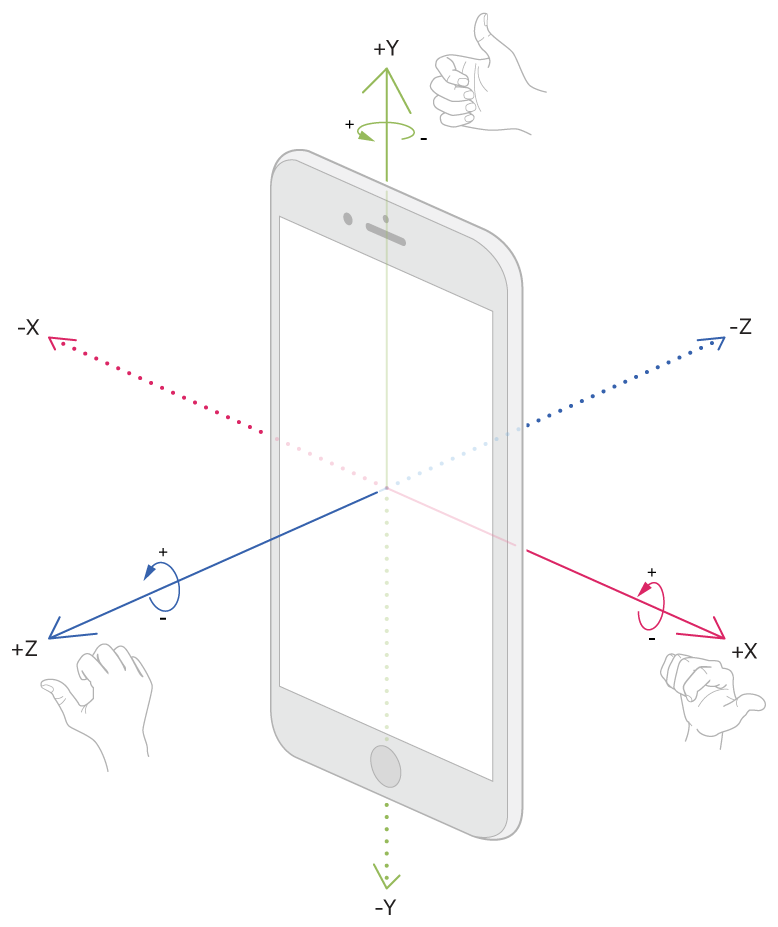
\includegraphics[height=.3\textheight]{../images/core-motion.png}
\caption{\label{fig:iphone-coordinates}The coordinate system of the IMUs in an Apple product \cite{appledocumentation} }
%https://developer.apple.com/documentation/coremotion/getting\_raw\_gyroscope\_events
\end{center}
\end{figure}

We can convert between these two rotation frames through a set of rotation matrices. We will use the yaw-pitch-roll Tait-Bryan angle convention often used to define the orientation of an aircraft (see Fig.~\ref{fig:aircraft-axes}). In this convention $\alpha$ represents yaw (i.e. anti-clockwise rotation about the $z$-axis), $\beta$ represents pitch (i.e., anti-clockwise rotation about the $y$ axis in the frame resulting from the yaw rotation), and $\gamma$ represents roll (i.e., anti-clockwise rotation around the $x$ axis in the frame resulting from the yaw and pitch rotations).

\begin{figure}
  \begin{center}
  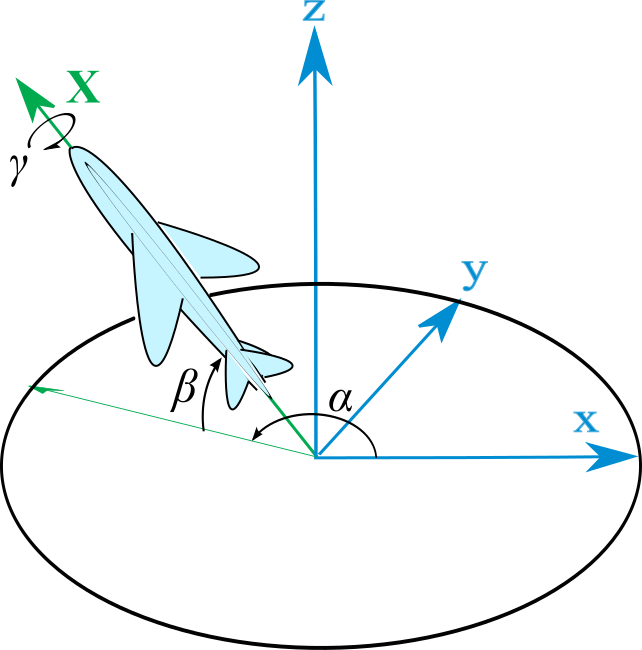
\includegraphics[width=.3\textwidth]{../images/plane-with-enu-embedded-axes.png}
  \caption{\label{fig:aircraft-axes}The Tait-Bryan angles that define an aircrafts orientation. Image adapted from \cite{wikipedia:angles}} 
  \end{center}
\end{figure}

Thus, motion in the global coordinate frame can be transformed into the phone's inertial frame with the following rotation matrices

\def\ca{\cos{\alpha}}
\def\sa{\sin\alpha}
\def\cb{\cos\beta}
\def\sb{\sin\beta}
\def\cg{\cos\gamma}
\def\sg{\sin\gamma}

\begin{align}
\begin{pmatrix}
X \\ Y \\ Z
\end{pmatrix}
&= R(\alpha, \beta, \gamma) 
\begin{pmatrix}
  x \\ y \\ z
\end{pmatrix}
%
\\&= R(0, 0, \gamma) R(0, \beta, 0) R (\alpha, 0 , 0) 
\begin{pmatrix}
  x \\ y \\ z
\end{pmatrix}
%
\\&= R(0, 0, \gamma) R(0, \beta, 0) R (\alpha, 0 , 0) 
\begin{pmatrix}
  x \\ y \\ z
\end{pmatrix}
%
\\&=
\begin{pmatrix}
  \cg & 0 & \sg \\
  0 & 1 & 0 \\
  -\sg & 0 & \cg
\end{pmatrix}
\begin{pmatrix}
  1 & 0 & 0 \\
  0 & \cb & -\sb \\
  0 & -\sb & \cb \\
\end{pmatrix}
\begin{pmatrix}
  \ca & -\sa & 0 \\
  \sa & \ca & 0 \\
  0 & 0 & 1
\end{pmatrix}
\begin{pmatrix}
  x \\ y \\ z
\end{pmatrix}
\\&= 
\begin{pmatrix}
\ca\cg-\sa\sb\sg & -\sa\cg - \ca\sb\sg & \cb\sg \\ 
\sa\cb & \ca\cb & -\sb \\
-\sa\sb\cg - \ca\sg & -\ca\sb\cg + \sa\sg & \cb\cg
\end{pmatrix}
\begin{pmatrix}
  x \\ y \\ z
\end{pmatrix}
\label{eq:rotationmatrix}
\end{align}

The rotation from the $XYZ$ frame to the $xyz$ frame can be achieved by

\begin{equation}
\begin{pmatrix}
x \\ y \\ z
\end{pmatrix}
=
R^T(\alpha, \beta, \gamma)
\begin{pmatrix}
X \\ Y \\ Z
\end{pmatrix}
\end{equation}

owing to the fact that $R$ is an orthogonal matrix, and that for any orthogonal matrix $R$, $R^{-1} = R^T$. In general, the transpose of a matrix is less computationally expensive to determine than its inverse.

As the body moves through space, it rotates, and its total orientation changes. The motion can be pictured as if the IMU is sitting on the axis of a slowly moving helicopter-like blade on top of the vehicle. That is, the vehicle moves linearly, but the IMU rotates at a constant rate. The rotation of the body about the $X-$, $Y-$, and $Z-$axes is detected by a MEMS chip with a gyroscope in each of those axes. The MEMS chip produces a reading for each axis (i.e., $\omega_X, \omega_Y$, and $\omega_Z$) every sample period $dt$. The rotation in yaw, pitch, and roll directions ($\delta\alpha, \delta\beta$, and $\delta\gamma$ respectively) are given by

\begin{align}
\begin{pmatrix}
\delta \alpha \\
\delta \beta \\
\delta \gamma 
\end{pmatrix}
=
\begin{pmatrix}
  \omega_Z \\
  \omega_Y \\
  \omega_X
\end{pmatrix}
dt
\end{align}

The total rotation $R_t$ at time $t$ of the body after the gyroscope update is then 

\begin{equation}
R_t = R(\delta \alpha, \delta\beta, \delta\gamma) R_{t-dt}
\end{equation}

$R_t$ is a $3 \times 3$ matrix, but only has three degrees of freedom (i.e., $\alpha, \beta$, and $\gamma$). Rather than tracking all nine elements of $R_t$, we can calculate the values of $\alpha, \beta$, and $\gamma$ at every time step from $R_t$ by exploiting several trigonometric identities of some of the elements.

\begin{align}
   R(\alpha, \beta, \gamma) 
  &=
  \begin{pmatrix}
    r_{11} & r_{12} & r_{13} \\
    r_{21} & r_{22} & r_{23} \\
    r_{31} & r_{32} & r_{33}\\
  \end{pmatrix}
  \\&= 
  \begin{pmatrix}
  \ca\cg-\sa\sb\sg & -\sa\cg - \ca\sb\sg & \cb\sg \\ 
  \sa\cb & \ca\cb & -\sb \\
  -\sa\sb\cg - \ca\sg & -\ca\sb\cg + \sa\sg & \cb\cg
  \end{pmatrix}
  \end{align}

\begin{align}
\frac{\sa}{\ca} &= \frac{r_{21}}{r_{22}} \\
-\sin\beta &= r_{23} \\
\frac{\sg}{\cg} &= \frac{r_{13}}{r_{33}}
\end{align}

\begin{align}
  \alpha &= \mathrm{atan2}(r_{21}, r_{22})\\
  \beta &= \mathrm{asin}(-r_{23}) \\ 
  \gamma &= \mathrm{atan}(r_{13}/r_{33})
\end{align}

The domain of $\beta$ and $\gamma$ are both $(-\pi/2, \pi/2)$, and the domain of $\alpha$ is $(-\pi, \pi]$. Therefore for software applications a function such as \texttt{arctan2} that can return values between $-\pi$ and $\pi$ needs to be used for calculating $\alpha$.

The system is degenerate when the device is vertical (i.e., $Y$ is in the $z$ direction), as there are infinitely many values of $\alpha$ and $\gamma$ that will result in that transformation. At device configurations near this orientation, this method suffers from numerical instability and is generally suboptimal. These methods are the most stable for applications where the screen of the phone almost parallel to the surface of the earth.

In order to model a device free from any numerical instabilities, one might investigate using a more mathematically complex approach using quaternions \cite{quaternion1, quaternion2}. This approach was not adopted in this work due to the added mathematical complexity, especially in linearizing the state-evolution equations in the Kalman Filter described below.

\section{Principle of a Kalman Filter}

GNSS sensors enjoy the ability to estimate a position almost anywhere on earth's surface. Unfortunately, they have relatively slow bandwidth (\SI{1}{Hz} for an iPhone's GNSS sensor), and fairly low precision (between five and ten meters for an iPhone GNSS sensor). The accuracy can further be reduced when there is no direct line of sight between the GNSS receiver and at least four satellites.

On the other hand, inertial sensors enjoy low noise and high bandwidth. For example, the CoreMotion APIs on an iPhone allow data to be extracted as fast as 100 samples per second, and the noise of the iPhone accelerometers and gyroscopes are about \SI{60}{\micro g/\sqrt{Hz}} and \SI{8}{mdeg/s/\sqrt{Hz}} respectively (see a later section in this paper on sensor characterization). However, inertial sensors suffer from a relatively large offset that can drift over time. Error in the gyroscopes will cause errors in the estimate of the orientation of the IMU, and errors in the accelerometer will cause errors in the velocity estimate, which in turn cause errors in the position estimate. These errors grow as time $t$ increases. 

Take for an example an error $\Delta a$ in the $x$-accelerometer. The error in the position estimate $\Delta x$ can be calculated

\begin{equation}
\Delta x = \frac{1}{2}\Delta a t^2
\end{equation}

Take for example, an accelerometer whose offset has drifted by \SI{100}{\micro g}. After one minute, the position error has grown to a modest \SI{1.77}{m}. However, after ten minutes, the error has grown to an unacceptably large \SI{177}{m}!

In order to bound this error, the predictions of an IMU are often aided by GNSS updates by means of some filter to produce a highly accurate estimate of the position and orientation at any time (see Table \ref{table:fusion}). Several varieties of filters have been developed \cite{mahony, madgwick, mahony2}. For the purposes of this work, we will use an Extended Kalman filter (EKF), which allows almost-optimal fusing of various sensors while also handling nonlinear dynamics. When modeling a purely linear system, the EKF reduces to an ordinary Kalman Filter, which has been shown to have optimal performance \cite{kalman}. Note that the EKF has some shortcomings, such as only being accurate to first-order expansions of the nonlinear equation. An unscented Kalman filter uses a slightly different approach to achieve third-order accuracy (in Taylor expansions) \cite{unscented}. 

\begin{table}
\centering
\begin{tabular}{| l || c | c | c |}
  \hhline{----}
  Characteristic & IMU only & GPS only & Sensor fusion \\\hhline{|=#=|=|=|}
  Bandwidth & fast & slow & fast \\\hline 
  Noise performance & good & poor & good \\\hline 
  Drift & unstable & stable & stable \\\hline  
\end{tabular}
\caption{\label{table:fusion} By using a carefully designed filter, a sensor-fusion technique provides state estimates using the best qualities of each constituent sensor.}
\end{table}

The algorithm of a Kalman filter is represented in Fig. \ref{fig:kalman-flowchart}. First, the user determines the state variables (both hidden and visible) $\vec{mu}$ that will be utilized by the filter. For this work, these variables are position, velocity, and orientation. The user also derives the equation $f(\vec{\mu}, \vec{u}$) which govern the system's evolution in time as well as the system's response to external stimulus (in our case, rotation rate and acceleration). Next, the user creates an estimate of how the uncertainty in the state variables grows with each time step and represents this with a square matrix $Q$ with the same height as $\vec{\mu}$. The characterization of $Q$ is discussed in a later section of this work.

\begin{figure}
  \centering
  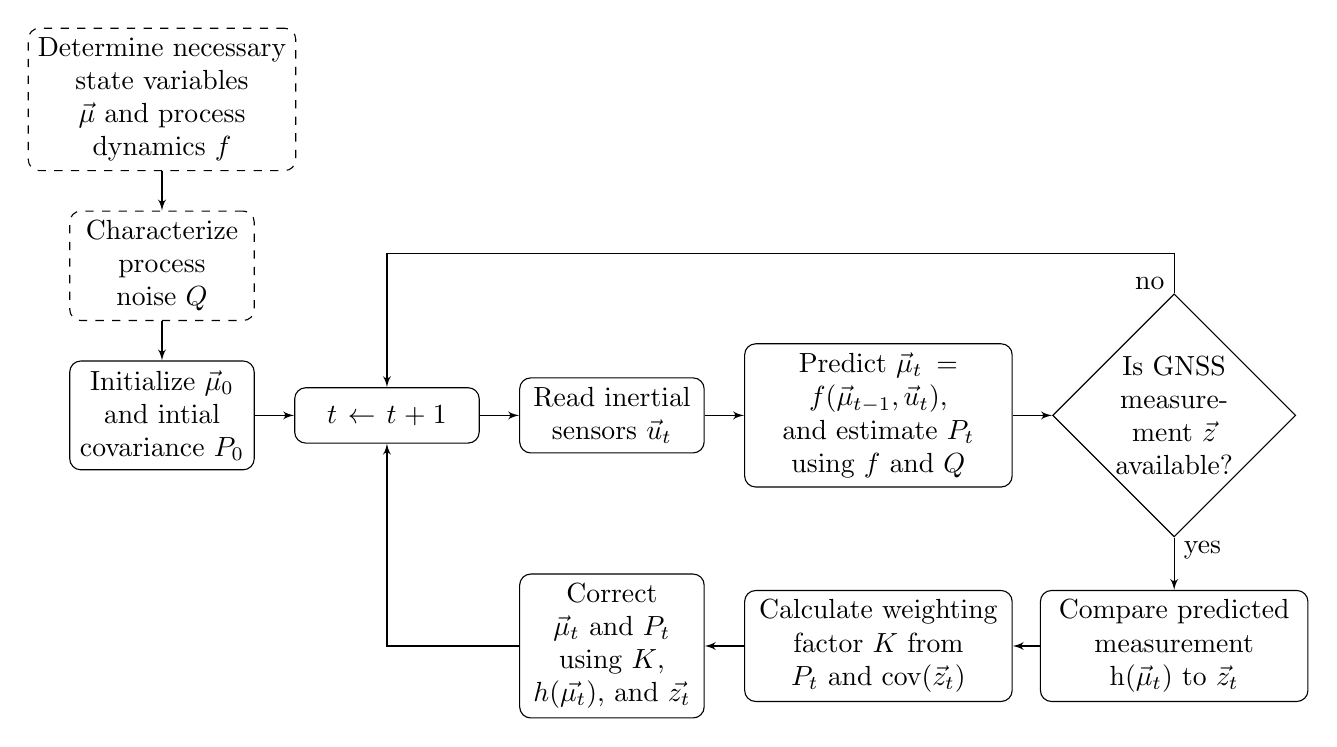
\begin{tikzpicture}
[
decision/.style={diamond, draw, text width=4.5em, text badly centered, node distance=0.5cm, inner sep=0pt},
                    block/.style   ={rectangle, draw, text width=6em, text centered, rounded corners, minimum height=4em, minimum height=2em},
					wide/.style   ={text width=9em},
                    cloud/.style   ={draw, ellipse, minimum height=2em},
                    line/.style    ={draw,-latex'},
                    node distance = .5cm, 
                    auto]

\node[block] (init) {Initialize $\vec{\mu}_0$ and intial covariance $P_0$};

\node[block, right=of init] (update) {$t \leftarrow t + 1$};

\node[block, dashed, above=of init] (characterize) {Characterize process noise $Q$};

\node[block, dashed, wide, above=of characterize] (determine) {Determine necessary state variables $\vec{\mu}$ and process dynamics $f$};

\node[block, right=of update] (odometry) {Read inertial sensors $\vec{u}_t$};
\node[block, wide, right=of odometry] (predict) {Predict $\vec{\mu}_{t} = f(\vec{\mu}_{t-1}, \vec u_t)$, and estimate $P_{t}$ using $f$ and $Q$};

\node[decision, right=of predict] (correct?) {Is GNSS measurement $\vec{z}$ available?};


\node[block, wide, below=1.3cm of predict] (gain) {Calculate weighting factor $K$ from $P_{t}$ and cov($\vec{z}_t$)};
\node[block, wide] at (gain -| correct?) (compare) {Compare predicted measurement h($\vec{\mu}_{t}$) to $\vec{z}_t$};

\node[block, left=of gain] (correct) {Correct $\vec{\mu}_{t}$ and $P_{t}$ using $K$, $h(\vec{\mu_t})$, and $\vec{z_t}$};

\path[line] (characterize) -- (init);
\path[line] (init) -- (update);
\path[line] (determine) -- (characterize);
\path[line] (update) -- (odometry);
\path[line] (odometry) -- (predict);
\path[line] (predict) -- (correct?);

\path[line] (correct?.north) -- ++ (0, .5) node[near start] {no} -| (update);
\path[line] (correct?) -- (compare) node[near start] {yes};
\path[line] (compare) -- (gain);
\path[line] (gain) -- (correct);
\path[line] (correct) -| (update);
  \end{tikzpicture}
  \caption{\label{fig:kalman-flowchart} A flowchart illustrating the algorithm of the Kalman filter}
\end{figure}

The filter itself is initiated with initial estimates of the state $\vec{\mu}_0$ and state uncertainty in the covariance matrix $P_0$ where $p_{ij}=\mathrm{cov}(\mu_i, \mu_j)$. Unlike an IMU-only system, where the system evolution is unstable and highly sensitive to initial conditions, the EKF is less sensitive to errors in initial conditions due to the GPS updates that occur in the filter. Large values in $P_0$ indicate large uncertainty in the initial state estimate $\vec{\mu}_0$, and instruct the filter to rely heavily on the GPS updates to estimate $\vec{\mu}$.

The filter then begins its main loop. At every time step, the filter gathers measurements $\vec{u}$ from the IMU, and uses them to estimate how the state has evolved since the last time step. The filter also linearizes $f(\vec{\mu}, \vec{u})$ to calculate a Jacobian matrix $F$


\begin{equation}
  F = \begin{pmatrix}
  \dfrac{\partial \mu_{1,t}}{\partial \mu_{1, t-1}} & \ldots &\dfrac{\partial \mu_{1,t}}{\partial \mu_{n, t-1}} \\
  \vdots & \ddots & \vdots \\
  \dfrac{\partial \mu_{n,t}}{\partial \mu_{1, t-1}} & \ldots & \dfrac{\partial \mu_{n,t}}{\partial \mu_{n, t-1}} \\
  \end{pmatrix}
  \end{equation}

The last step of the predict step is to update it's estimate of the covariance of the system. It does so by adding the process noise $Q$ to the covariance of the previous timestep after it has passed through the state dynamics.

\begin{equation}
P_t = FP_{t-1}F^T + Q
\end{equation}

If there are no new data from the GNSS sensor, then the calculations for this timestep are complete, and the filter awaits input from the next timestamp. However, if the GNSS has a new measurement $\vec{z}_t$, then the filter uses it to reduce the uncertainty of $\vec{\mu}_t$. Toward this end, the filter estimates what GNSS measurement it expects via the function $h(\vec{\mu}$). In this work, the GPS measurements $\vec z$ are in the same coordinate frame as the position state variables in $\mu$. This allows $h(\vec{\mu}) = H\vec{\mu}$ where $H$ is a $3 \times \mathrm{dim}(\vec{\mu})$ matrix with ones corresponding to the placements of $x$, $y$, and $z$ in $\vec{\mu}$ and zeros elsewhere. The error between the actual measurement and the prediction of the measurement is given by the residual $y$

% Explain H
% Explain K
\begin{equation}
y = \vec{z_t} - H\vec{\mu}_t
\end{equation}

In general, updating the state by the full residual would cause the system to overcorrect, since the GNSS data contains significant noise. To mitigate the amount of noise introduced to the system by correcting the residual, the residual is scaled by a gain factor $K$. 

\begin{equation}
K = P_t H^T (\mathrm{cov}(\vec{z}) + H P_t H^T)^{-1}
\end{equation}

If $K$ is small, then the system relies heavily on the time evolution from the equations of motion. If $K$ is large, then the filter relies heavily on the values of the GNSS update. The filter also uses the covariance in $\mathrm{cov}(\vec{z})$ to reduce the overall uncertainty in $P$. Note that the literature typically refers to $\mathrm{cov}(\vec{z})$ as $R$, but we shall refer to it henceforth as $S$ in this text to avoid confusion with the rotation matrices (the literature makes use of $P$, $Q$, and $R$, thus $S$ is the next letter in the alphabet to use). 

Thus, the optimal correction equations are given by

\begin{align}
\vec{\mu}_t & \leftarrow \vec{\mu}_t + K (\vec{z_t} - H\vec{\mu}_t) \\
P_t & \leftarrow (I - KH) P_t (I - KH)^T + KSK^T
\end{align}

After the correction, the timestep is incremented, and the filter awaits new data from the inertial sensors.



\section{Kalman Filtering of Simulated Motion in One Dimension}

In order to build up our model, we took a number of incremental intermediate steps in order to catch any errors in the code early. A large number of simulation cases (at least ten) were performed, but only the few most interesting and pertinent studies are reported herein. First, a Kalman filter was programmed to model a simulated particle moving along one dimension. The moved a total of \SI{10}{m} over the course of \SI{60}{s}, and particle's true position was given by

\begin{align}
  x(t) = \SI{10}{m}\left(1 - \cos\left( \frac{2\pi t}{\SI{2}{min}}\right)\right) / 2
\end{align}

The IMU consisted of a single accelerometer oriented in the direction of motion with a sampling rate $f_s$ of \SI{10}{Hz} and a noise $\sigma_a$ of \SI{1}{mg/\sqrt{Hz}}. The GNSS receiver had a sampling rate of \SI{1}{Hz} and an rms error $\sigma_z$ of \SI{1}{m}.

The properties of the EKF were

\begin{align}
\vec{\mu} &= \begin{pmatrix} x & v \end{pmatrix}^T \\
  Q & = \begin{pmatrix}
    \sigma_a \sqrt{f_s} dt^2/2 & 0 \\
    0 & \sigma_a \sqrt{f_s} dt
  \end{pmatrix}^2 \\
  u &= a[t] \\
  f(\vec{\mu}, \vec{u}) &= \begin{pmatrix}
    1 & dt \\ 0 & 1
  \end{pmatrix} \vec{\mu} 
  + \begin{pmatrix} 
    dt^2/2 \\ dt
  \end{pmatrix} u
  \\
  S &= \sigma_z^2 \\ 
H &= \begin{pmatrix} 1 & 0 \end{pmatrix} \\
  P_0 &= Q + R
\end{align}

Figure \ref{fig:1d-accelerometer-results} shows the output of this filter given the simulated data described above. The outputs of the system guided by either the IMU or GNSS alone are also shown, as well as the true position of the particle. The width to the green trace illustrates the $\pm 1\sigma$ error bars (i.e., the filter estimates particle is 68\%-likely to be within the green region). The 1-sigma uncertainty can estimated for all of the state variables at each timestep by taking the square root of the diagonals in the $P$ vector. 

\begin{figure}[hbt]
  \centering
  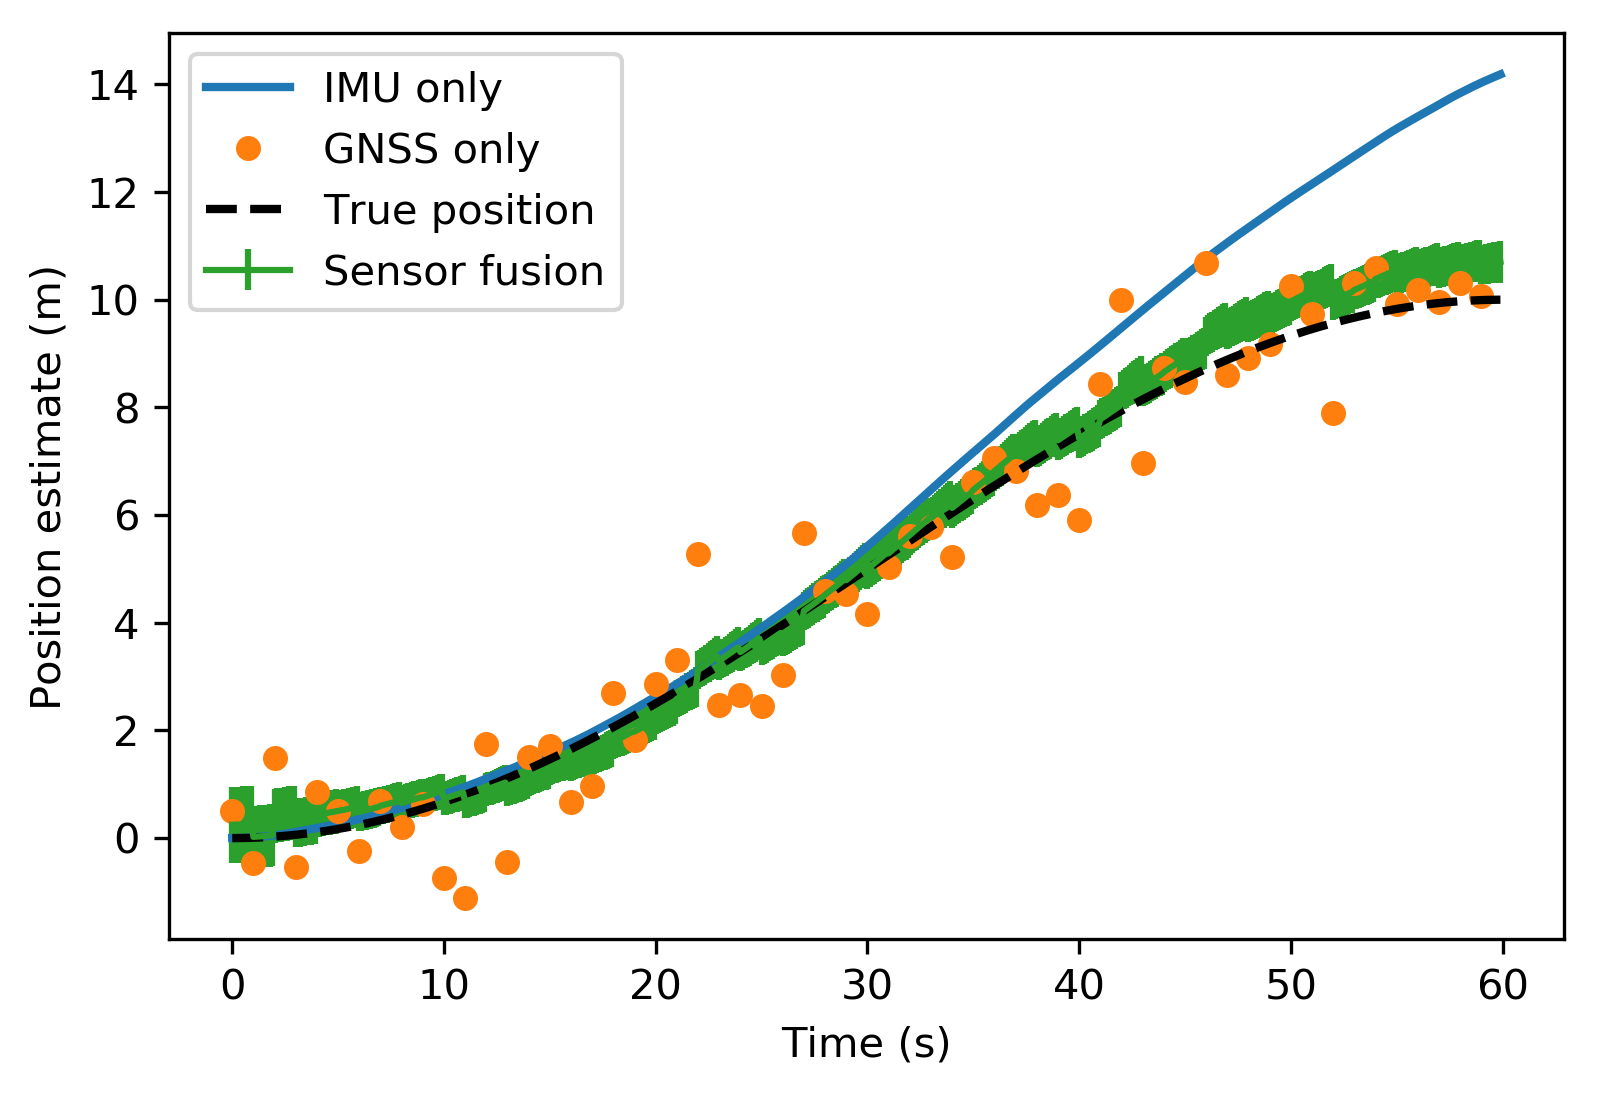
\includegraphics[width=.5\textwidth]{../images/1d-accelerometer-simulation.png}
  \caption{\label{fig:1d-accelerometer-results} The results of the simulated particle accelerating in one dimension}
\end{figure}

The IMU-only system experiences large amounts of drift relative to the true position, while the GNSS-only system suffers from large amounts of noise and limited bandwidth. 

The Kalman filter does a satisfactory job of merging the low drift of the GNSS data with the low noise of the accelerometer.

Next, we consider the same Kalman filter, but this time we simulate a GNSS outage from $t=\SI{10}{s}$ until $t=\SI{40}{s}$. The results of the Kalman filter are shown in Fig. \ref{fig:1d-accelerometer-results-wth-outage}

\begin{figure}[hbt]
  \centering
  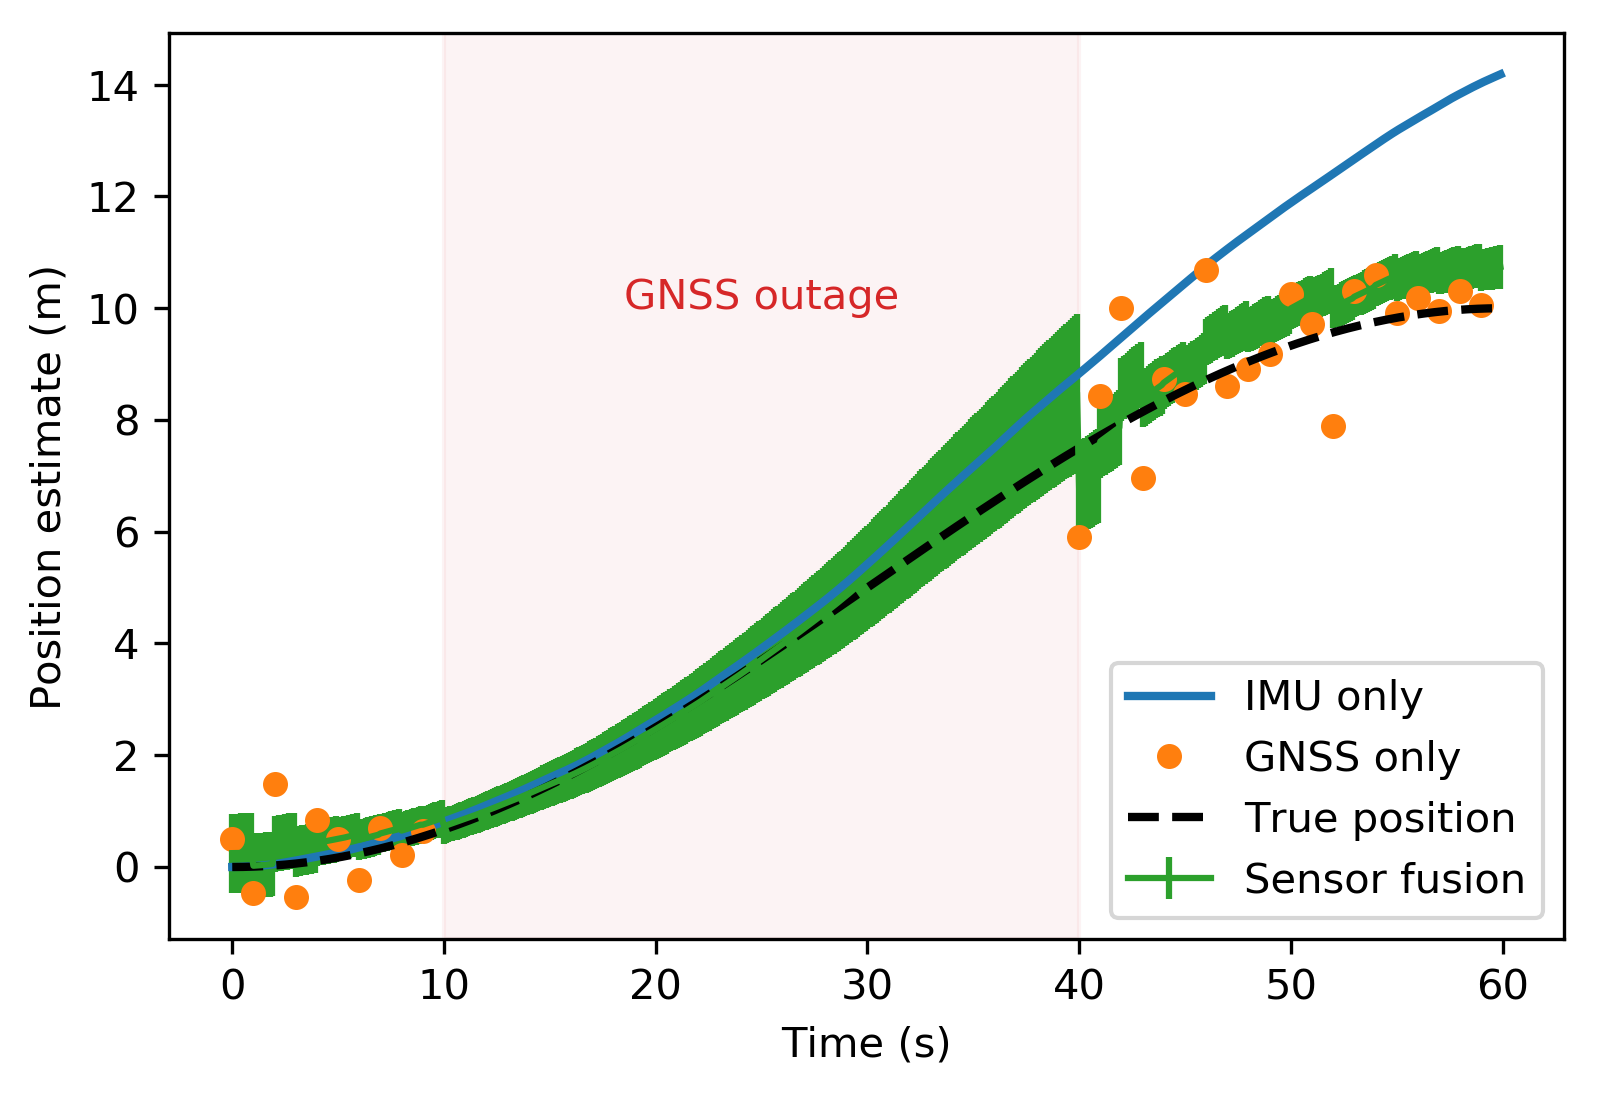
\includegraphics[width=.5\textwidth]{../images/1d-accelerometer-simulation-with-simulated-outage.png}
  \caption{\label{fig:1d-accelerometer-results-wth-outage} The results of the simulated particle accelerating in one dimension}
\end{figure}

In Fig.~\ref{fig:1d-accelerometer-results-wth-outage}, we see that the uncertainty of the Kalman-filter position state begins small, but when the GNSS updates become unavailable, the position estimate drifts relative to the true position, and the uncertainty grows. The Kalman filter's design allows it to realize that it has not received an update, and its error bars grow. In this iteration, the true position falls within the 1-sigma confidence interval during the entire outage, and when the GNSS data becomes available again, the filter quickly converges towards the correct value again. Towards the end of the simulation, the estimated position is a little larger than the true position, but this is due to both the accelerometer and the GNSS errors consistently pulling it in the positive direction.

\section{Kalman Filtering of Simulated Motion in Two Dimensions}

To simulate motion in two dimensions, an IMU with two accelerometers (in the $X$ and $Y$ device axes) and one gyroscope (in the $z = Z$ axis) was modeled. The true position of the device was given by

\begin{equation}
  \begin{pmatrix}
    x \\ y 
  \end{pmatrix}
  = d_{max} \left( 1 - \cos(2\pi t / T) \right) / 2
  \begin{pmatrix}
    \cos \theta \\ \sin \theta 
  \end{pmatrix}
\end{equation}

where $d_{max}$ was \SI{10}{m}, $\theta$ was $\pi/4$, and $T$ was \SI{2}{min}. The simulated IMU was subject to a rotation of $\Omega_Z$ = \SI{0.1\pi}{rad/s}, such that the axes of the accelerometers were constantly rotating with respect to the global reference frame. 

The accelerations $a_X$ and $a_Y$ of the $X$- and $Y$-axis accelerometers  and rotation $\omega_Z$ measured by the gyroscope were given by 

\begin{align}
\begin{pmatrix}
  a_X \\ a_Y
\end{pmatrix}
&=
\begin{pmatrix}
\ca & -\sa \\
\sa & \ca
\end{pmatrix}
\begin{pmatrix}
\ddot x \\ \ddot y
\end{pmatrix}
+
\begin{pmatrix}
w_X \\ w_Y
\end{pmatrix}
\\
\omega_Z &= \Omega_Z + w_Z
\end{align}

where $\ddot x$ and $\ddot y$ represent the second-order derivatives of x and y with respect to time (i.e., the true accelerations in those axes). The $w$ terms represent noise added to the system, and are Gaussian random variables. Both $w_X$ and $w_Y$ have an rms error of $\sigma_a \sqrt{f_s}$ where $\sigma_a$ is the characteristic noise of the accelerometers, and is assumed to be the same in the $X$ and $Y$ directions. $w_Z$ has an rms error of $\sigma_g \sqrt{f_s}$ where $\sigma_g$ is the characteristic noise of the gyroscope.

In this simulation, $f_s$ = \SI{10}{Hz}, $\sigma_a$ = \SI{1}{mg/\sqrt{Hz}}, $\sigma_g = \SI{1}{mrad/s/\sqrt{Hz}}$. The GNSS receiver had a sampling rate of \SI{1}{Hz} and an rms error $\sigma_z$ of \SI{1}{m} in both the $x$ and $y$ directions.

Note that these equations have neglected the Coriolis force and thus are slightly aphysical. As will be discussed in a further section, the omission of the Coriolis effect when filtering real sensor data will lead to errors. However, because no Coriolis forces are being added to the simulation, the Kalman filter will function well if its process equations do not include the Coriolis force.

\begin{align}
\vec{\mu} &= \begin{pmatrix} x & y & \dot{x} & \dot{y} & \alpha \end{pmatrix}^T \\
  Q & = \begin{pmatrix}
    \sigma_a \sqrt{f_s} dt^2/2 & 0 & 0 & 0 & 0 \\
    0 & \sigma_a \sqrt{f_s} dt^2/2 & 0 & 0 & 0 \\    
    0& 0 & \sigma_a \sqrt{f_s} dt & 0 & 0\\
    0 & 0 & 0 & \sigma_a \sqrt{f_s} dt & 0 \\
    0 & 0 & 0 & 0 &  \sigma_g \sqrt{f_s} dt 
  \end{pmatrix}^2 
\end{align}
\begin{align}
  \vec{u} &= \begin{pmatrix}
    a_X & a_Y & \omega_Z
  \end{pmatrix}^T 
\end{align}
\begin{align}
  f(\vec{\mu}, \vec{u}) &= \begin{pmatrix}
    1 & 0 & dt & 0 & 0\\ 0 & 1 & 0 & dt &0 \\
    0&0&dt&0&0 \\ 0&0&0&dt&0 \\
    0&0&0&0&1  
  \end{pmatrix} \vec{\mu} 
  + \begin{pmatrix} 
    \ca dt^2/2 & \sa dt^2 & 0 \\
    -\sa dt^2/2 & \ca dt^2  & 0 \\
    \ca dt & \sa dt & 0 \\
    -\sa dt & \ca dt0 & 0 \\
     0 & 0 & dt \\               
  \end{pmatrix} \vec u
  \\
  F & = \begin{pmatrix}
    1 & 0 & dt & 0 & (-\sa a_X  + \ca a_Y) \frac{dt^2}{2} \\
    0 & 1 & 0 & dt & (-\ca a_X  + -\sa a_Y) \frac{dt^2}{2} \\
    0 & 0 & 1 & 0 & (-\sa a_X  + \ca a_Y) dt \\
    0 & 0 & 0 & 1 & (-\ca a_X  + -\sa a_Y) dt \\ 
    0 & 0 & 1 & 0 & 1 
  \end{pmatrix}\\
  S &= \begin{pmatrix}
    \sigma_z^2 & 0 \\ 0 & \sigma_z^2
  \end{pmatrix} \\ 
H &= \begin{pmatrix} 1 & 0 & 0 & 0 & 0 \\ 0 & 1 & 0 & 0 & 0 \end{pmatrix} \\
  P_0 &= Q + R
\end{align}

Note that in this simulation, the element in the diagonal of $P_0$ corresponding to the uncertainty in yaw is set to $\pi^2$, indicating that we are very uncertain about our initial estimate in yaw.

\begin{figure}
  \centering
  \begin{subfigure}[b]{.35\textwidth}
    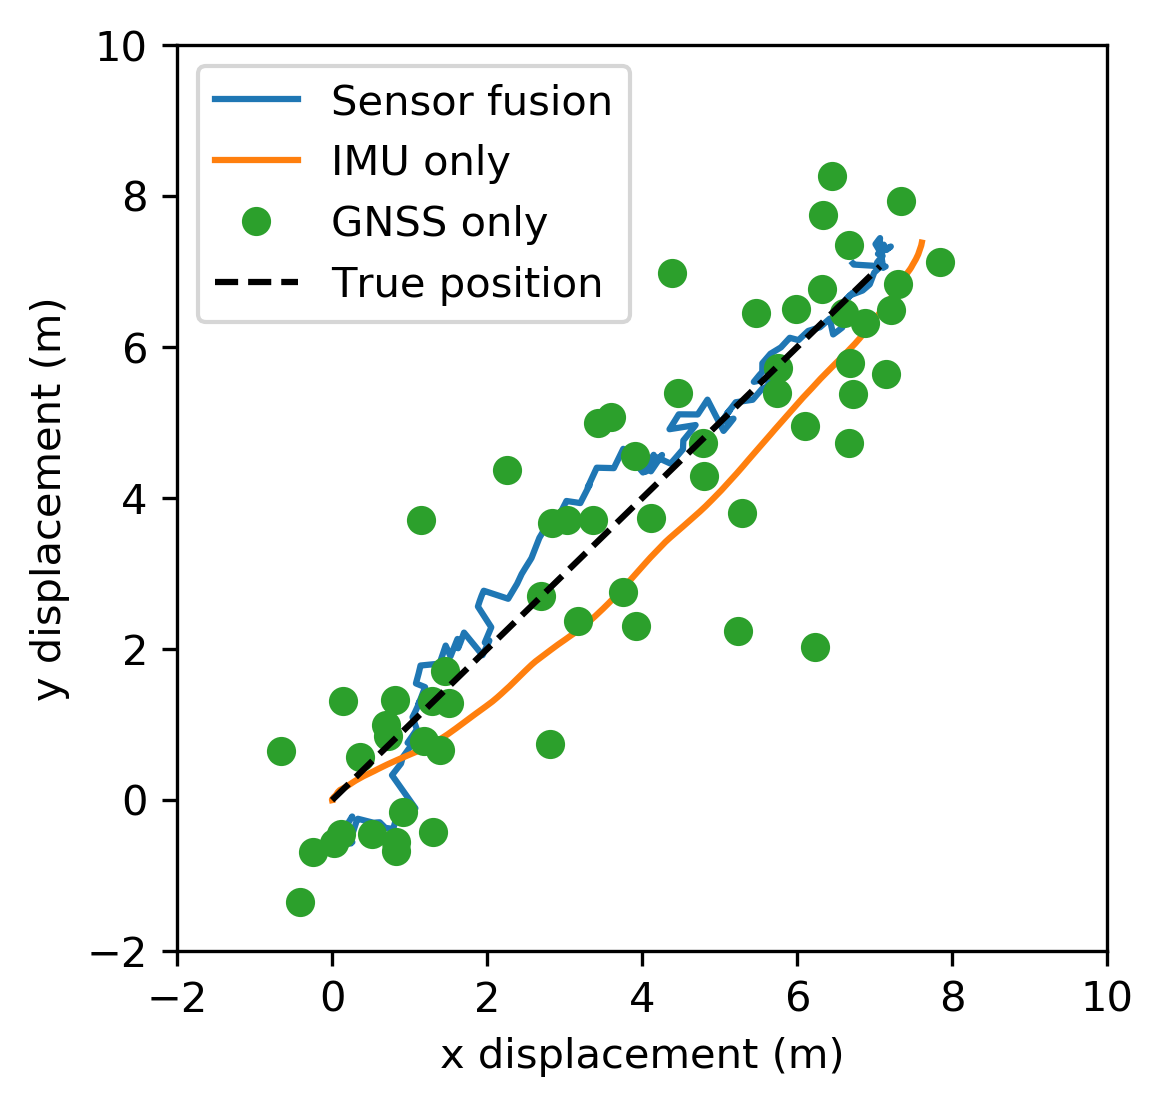
\includegraphics[width=\textwidth]{../images/position-with-initial-estimate-right.png}
  \end{subfigure}
  \begin{subfigure}[b]{.5\textwidth}
    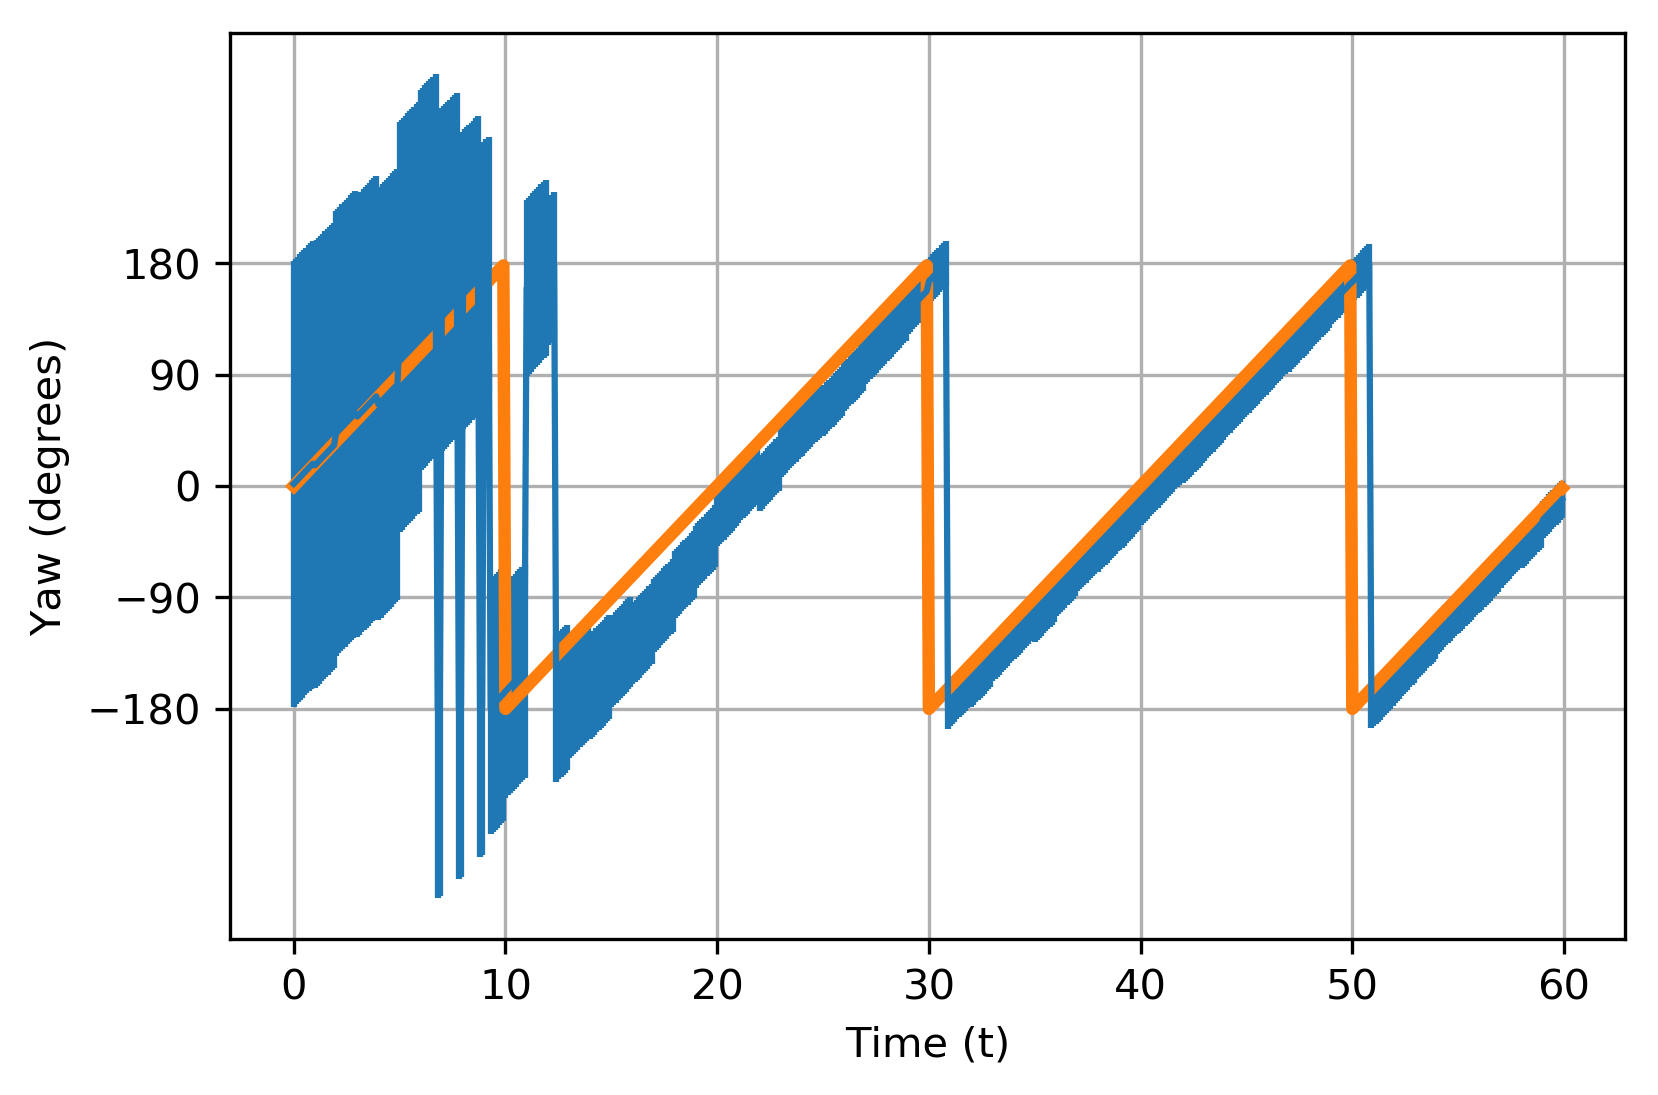
\includegraphics[width=\textwidth]{../images/yaw-with-large-initial-estimate-right.png}
  \end{subfigure}
  \caption{\label{ref:2d-correct-initial} Left: A top-down view of the object as it propagates. The object moves from the bottom left to the top right. The estimated motion of the IMU without GNSS updates, the GNSS updates, the Kalman-filter output, and the true position are all plotted. Right: The yaw (clockwise rotation from the x-axis about the z-axis) is plotted with respect to time.}
\end{figure}
%\section{Kalman Filter of iPhone Accelerometers to Determine Pitch and Roll}


Figure \ref{ref:2d-correct-initial} illustrates the dynamics of the object as the simulation evolves. The motion of the particle as seen in a top-down view is illustrated on the left side of Fig. \ref{ref:2d-correct-initial}, where the object moves from the bottom-left corner to the top-right corner of the chart. The right side of the figure illustrates the yaw estimate in the sensor-fusion algorithm over time. At the beginning of the simulation, the algorithm is told that the estimate for the yaw is $0 \pm \pi$ radians. As the Kalman filter evolves with time, this estimate is refined and the error bars become quite small (only a few degrees). Even though the GNSS data does not contain any angular measurements (a magnetometer, on the other hand, would), the GNSS data can still reduce the uncertainty in yaw due to the off-diagonal terms in the $F$ matrix. To understand how this is possible, consider the $P$ matrix, which is influenced by the $F$ matrix. The $P$ matrix contains the covariances between different variables in the state. So while there may be an uncertainty cloud in position (the rms error of the position is given by the diagonal term), the left-part of the cloud may be correlated with positive errors in yaw, and the right-part of the cloud may be correlated with negative errors in yaw. If the GNSS update tells the sensor that the true position is in the left part of the cloud, the filter learns not only that the position estimate needs to be correct to the left, but the yaw estimate needs to be increased to a larger value.

In the process of writing this report, we noticed that the IMU-only position seemed to veer right of the true position, while the sensor-fusion position seemed to veer left. This could be indicative of the rotation matrices being backwards (i.e., a rotation matrix rotation clockwise when the user intends for it to rotate anticlockwise). Several attempts were made to remedy this apparent error, but with no success.

The simulation was repeated, but in this test the initial estimate of yaw was intentionally wrong by $-\pi/2$ (an error resulting in the object to be oriented $90^\circ$ to the right). The results of this simulation are shown in Fig. \ref{ref:2d-wrong-initial}.

\begin{figure}
  \centering
    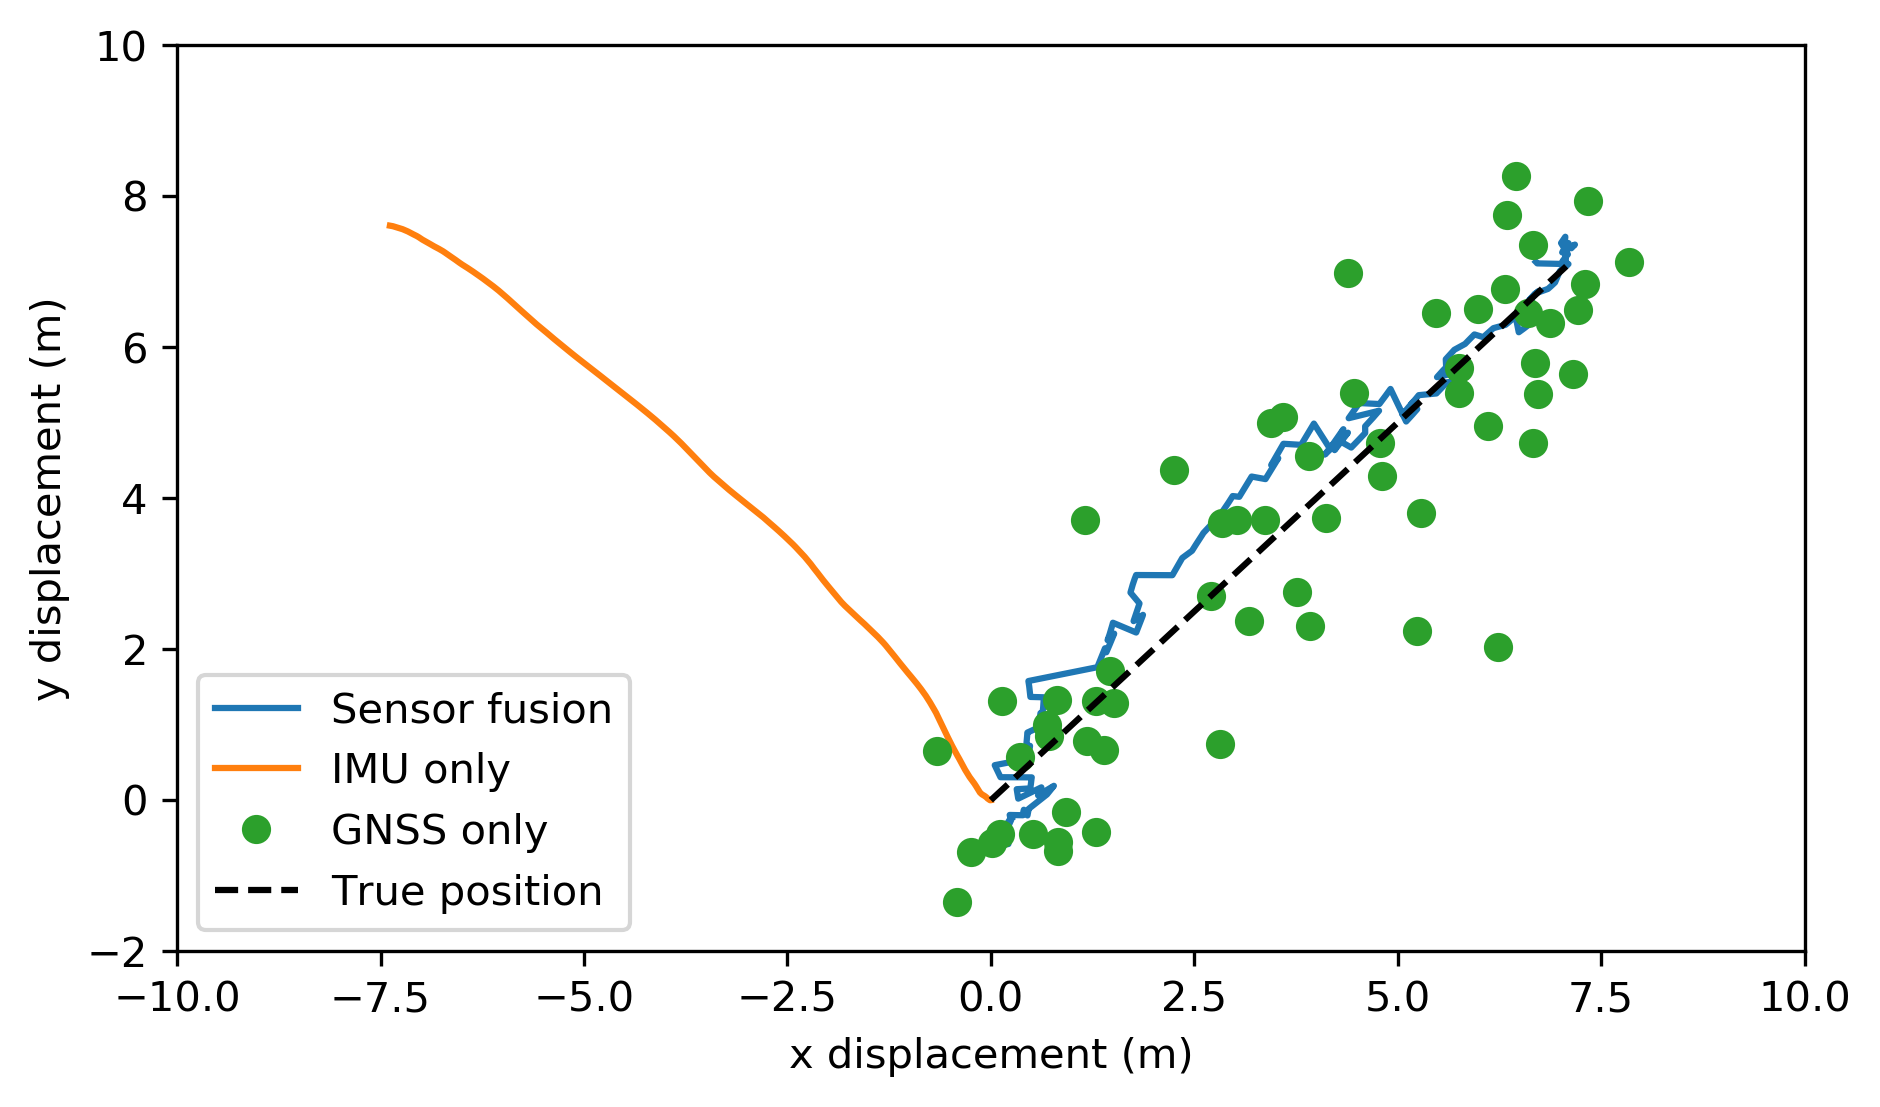
\includegraphics[height=2 in]{../images/position-with-initial-estimate-wrong.png}
    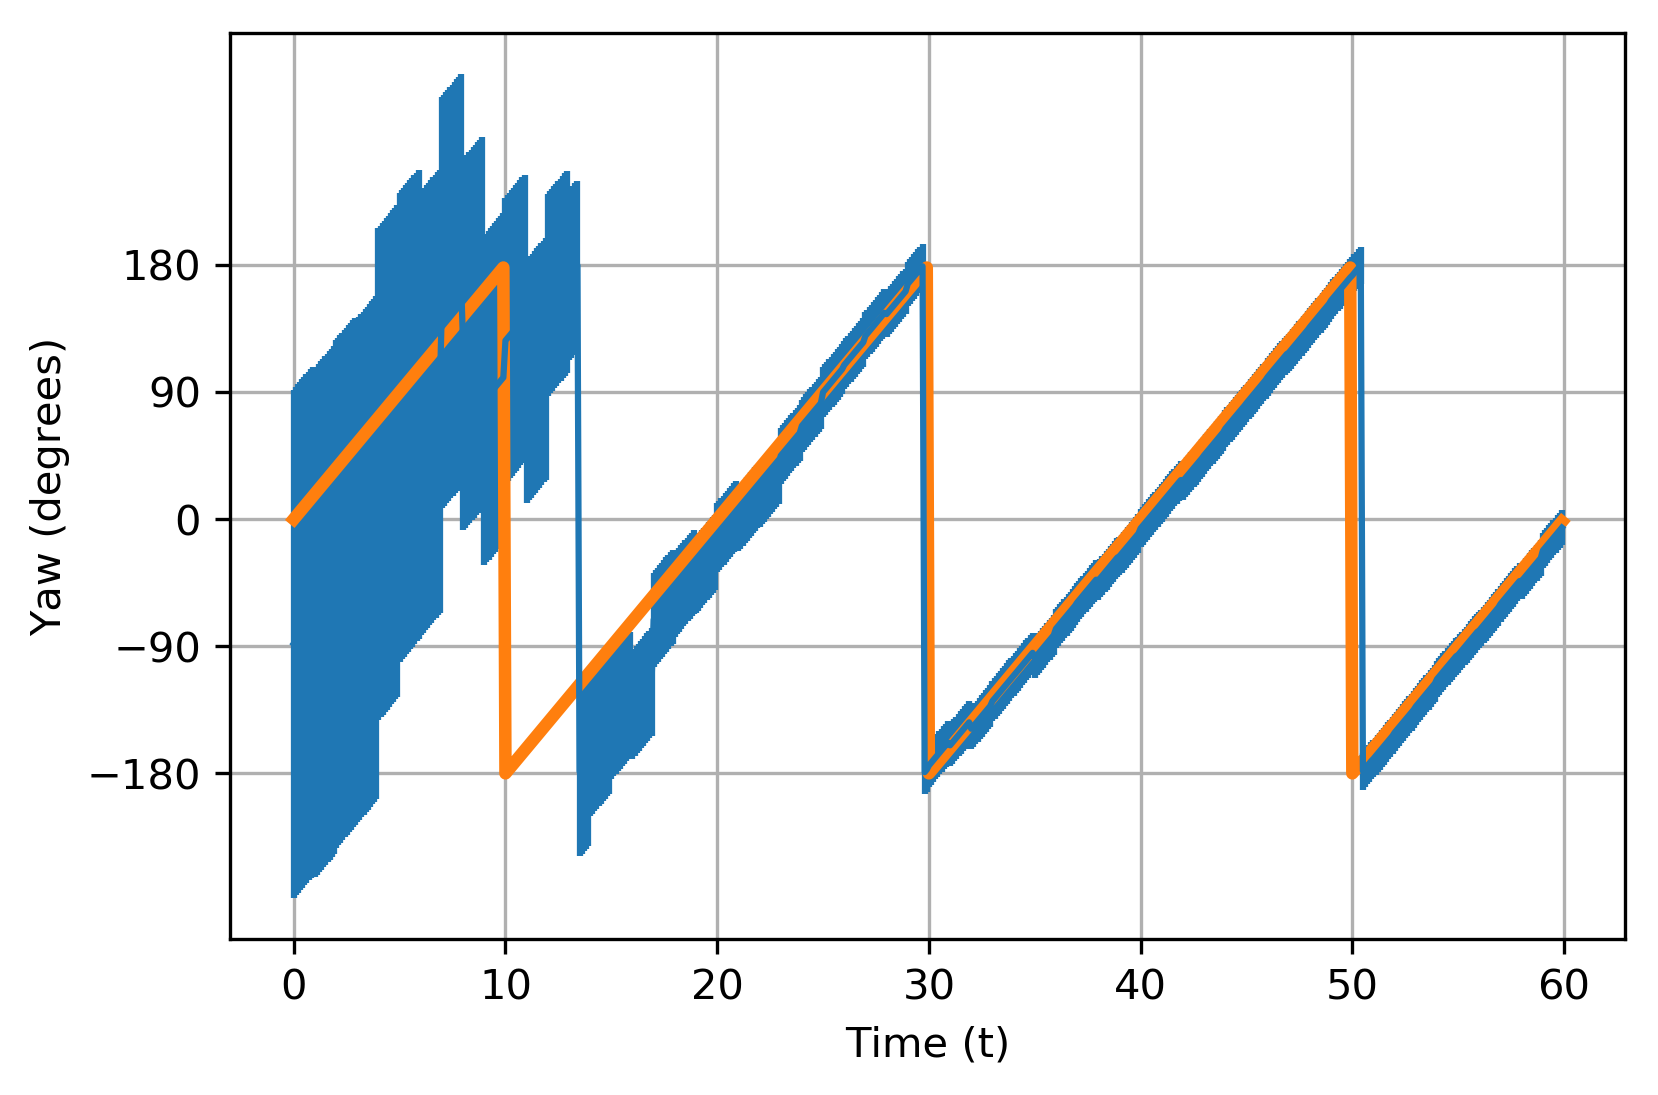
\includegraphics[height=2 in]{../images/yaw-with-large-initial-estimate-wrong.png}
  \caption{\label{ref:2d-wrong-initial}Left: A top-down view of the object as it propagates. In this simulation, the IMU received an incorrect initial estimate of the yaw. The true position of the object moves from the bottom center to the top right. The estimated motion of the IMU without GNSS updates, the GNSS updates, the Kalman-filter output, and the true position are all plotted. Right: The yaw (clockwise rotation from the x-axis about the z-axis) is plotted with respect to time.}
\end{figure}

Again, we see that the system seems to misinterpret the value of the yaw, such that a negative yaw induces a anticlockwise rotation about the Z axis, when it should be causing a clockwise rotation. Nevertheless, the Kalman filter still manages to cause the position and yaw estimates to converge to close of that of their true values, despite this apparent modeling error. The yaw error begins at $-90^\circ$ and diminishes to a few degrees by the end of the simulation.

\section{Simulating the Motion in 3D space}

We did not have a chance to create a simulation of the motion in 3D space. Instead, we prioritized getting actual data for the final project. As will be discussed in a further section, our implementation of the 3D Kalman Filter seems to have errors, and thus one of the next steps is to perform the simulation in 3D space with known forces to debug and troubleshoot the problem.

\section{Characterizing Noise and Bias Drift with the Allan-Variance Method}

The Apple API exposes the horizontal and vertical estimates for GNSS data. However, there is no publicly available documentation for the error performance of the IMU (nor does Apple even publish which IMU the iPhone uses!). In order to estimate the values to place into the $Q$ matrix for the real iPhone data, the noise of each sensor needs to be characterized.

The IEEE defines a standard method of characterizing gyroscope and accelerometer errors \cite{IEEEgyroscopecharacterization}. This is done by placing the IMU at rest on some stable, vibration-free surface. The IMU collects data for a long period of time (the requisite length of time is often a function of the bias-stability performance of the sensor; consumer-grade sensors need a few minutes to hours, military-grade sensors need weeks). Then, a statistical value called the Allan variance is calculated for a variety of integration times for each sensor. The Allan variance for a discrete signal $y[t]$ is given by

\begin{equation}
\mathrm{AVAR}(\tau) = \frac12 \left< (\bar{y}_{n+1} - \bar{y}_n )^2 \right>
\end{equation}

where 

\begin{equation}
  \bar{y}_n = \frac{dt}{\tau}\sum_{i = n\tau/dt}^{(n+1)\tau/dt} y[i]
\end{equation}

and represents the average value for all of the data in the $n$th bin of data of bin-duration $\tau$. It is also common to discuss the Allan deviation of a process, where the Allan deviation is the square root of the Allen variance (though it is common in the literature to refer to the a plot of the Allan deviation as an Allan-variance plot). The interpretation Allan deviation (ADev) for a given integration time $\tau$ is that the expected deviation between two consecutive averages of length $\tau$ is ADev($\tau$).

% TODO include figure of Allan deviation

On a log-log plot of the ADev($\tau$) vs $\tau$, the left hand side often is characterized by a long straight line with a slope (or exponent in linear plot) of -1/2. The intercept of this line with $\tau = \SI{1}{s}$ indicates the noise of the sensor. The right side of the curve often gives rise to lines that are somewhat less linear with a slope of 0, +1/2, or +1. The standards defined in \cite{IEEEgyroscopecharacterization} give a greater description of the physical processes that drive the long-term offset fluctuations that give rise to each of these different slopes). In an advanced implementation of a Kalman filter, six additional state variables would be used to track the bias offsets of the six IMU sensors. While the gyro noise and accelerometer noise would determine the values of the Q-matrix for the orientation and velocity states respectively, the gyro drift and accelerometer drift (as estimated from the right-hand side of the log-log graph) would be used to determine the values of the Q-matrix associating with the rate of change of the IMU-sensor drifts. 

The iPhone 8 to be characterized was placed on a flat surface and allowed to collect data for 2.5 hours. The time trace of the sensor offsets is shown in Fig. \ref{fig:imu-offset-traces}.

\begin{figure}
  \centering
  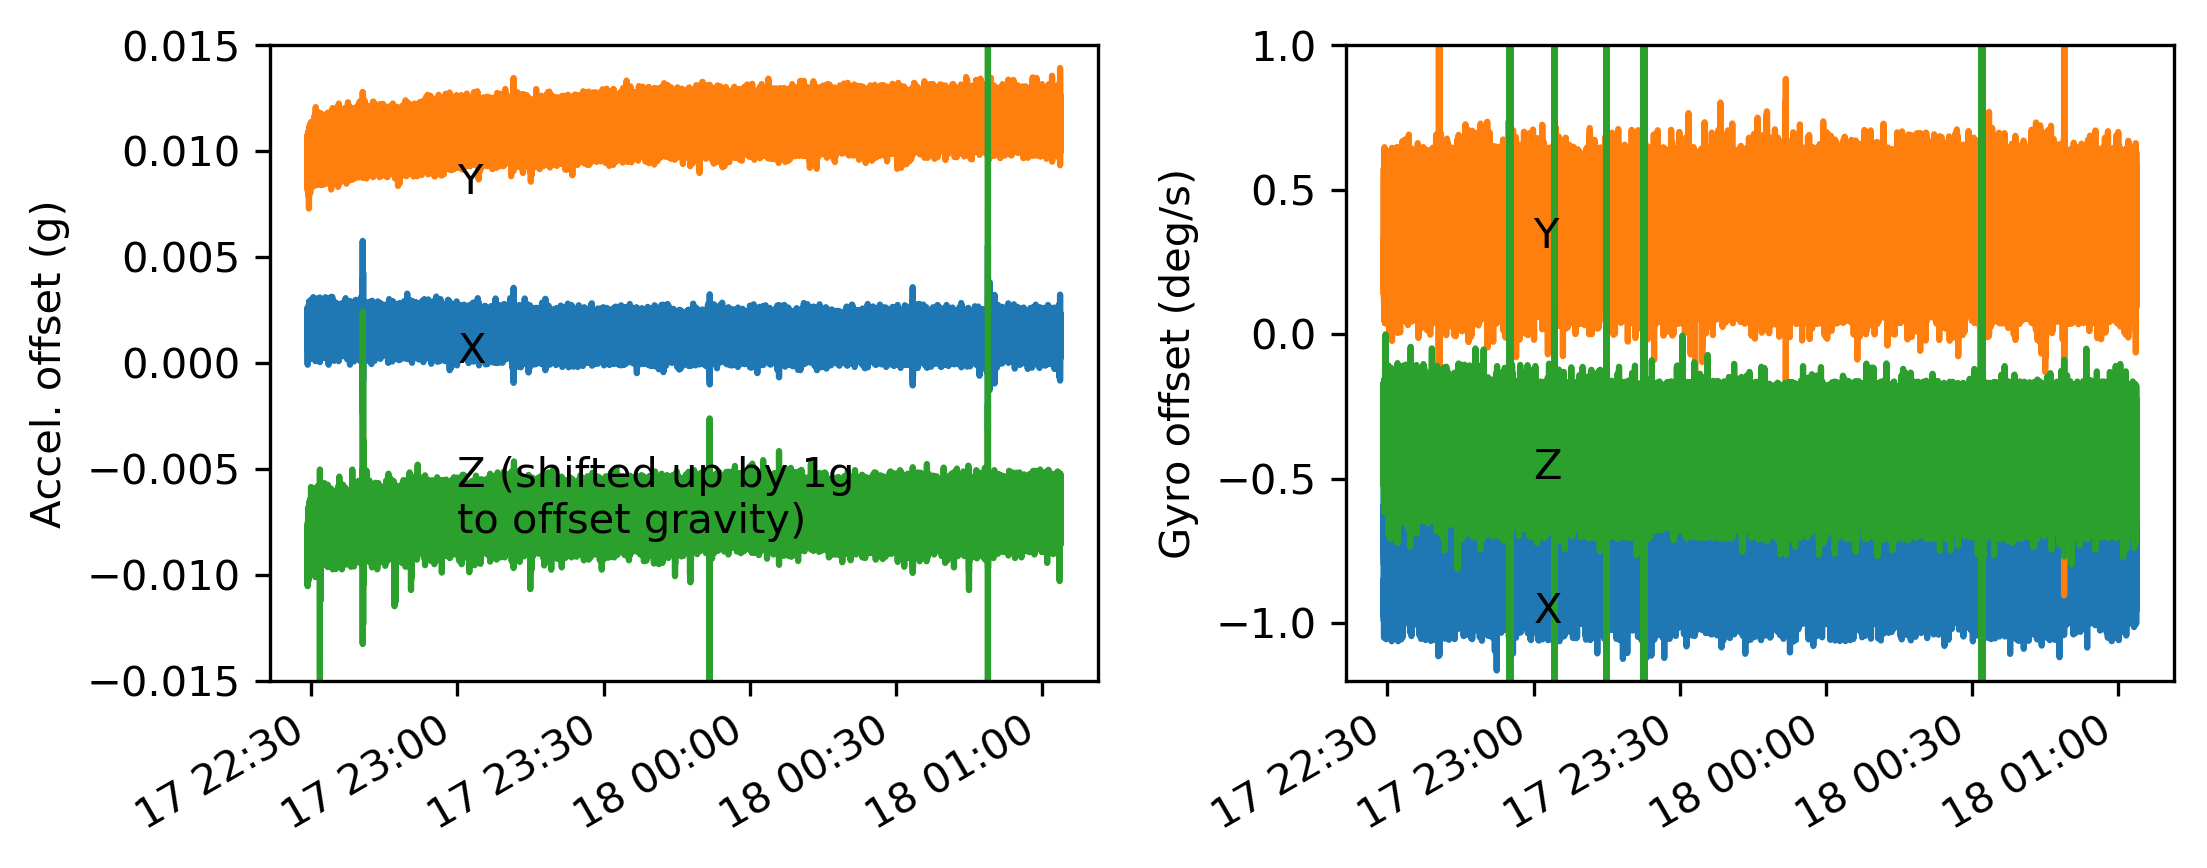
\includegraphics[width=\textwidth]{../images/time-trace-characterization2.png}
  \caption{\label{fig:imu-offset-traces} A 2.5-hour time trace for the sensor offsets over time. Note that the sensor drift is somewhat difficult to see as it is buried under the high noise when the sensor was sampled at 100 Hz}
\end{figure}

The Allan deviation plots for the data shown in Fig. \ref{fig:imu-offset-traces} are shown in Fig. \ref{fig:allan-deviation}. The Allan-deviation plots reveal that accelerometers all have a noise performance of \SI{60}{\micro g/\sqrt{Hz}} or better, and the gyroscopes have a noise performance of \SI{60}{mdeg/\sqrt{Hz}} or better. The Allan deviation for the IMU sensors decreases with increasing integration time until $\tau$ is about \SI{30}{s}. This indicates that the offset does not drift a visible amount (relative to the sensor noise) under short time scales, but it does drift significantly (relative to the sensor noise) for long time scales. For short trajectories (a few minutes), the offset can be measured at the beginning of the trajectory (before motion begins), and that offset can be used to null out any bias for the remainder of the tests. However, the drift is significantly large that the offset may vary over the course of several hours, so the offset from a test in the morning cannot in general be used to correct the bias error for a test in the evening.

\begin{figure}
  \centering
  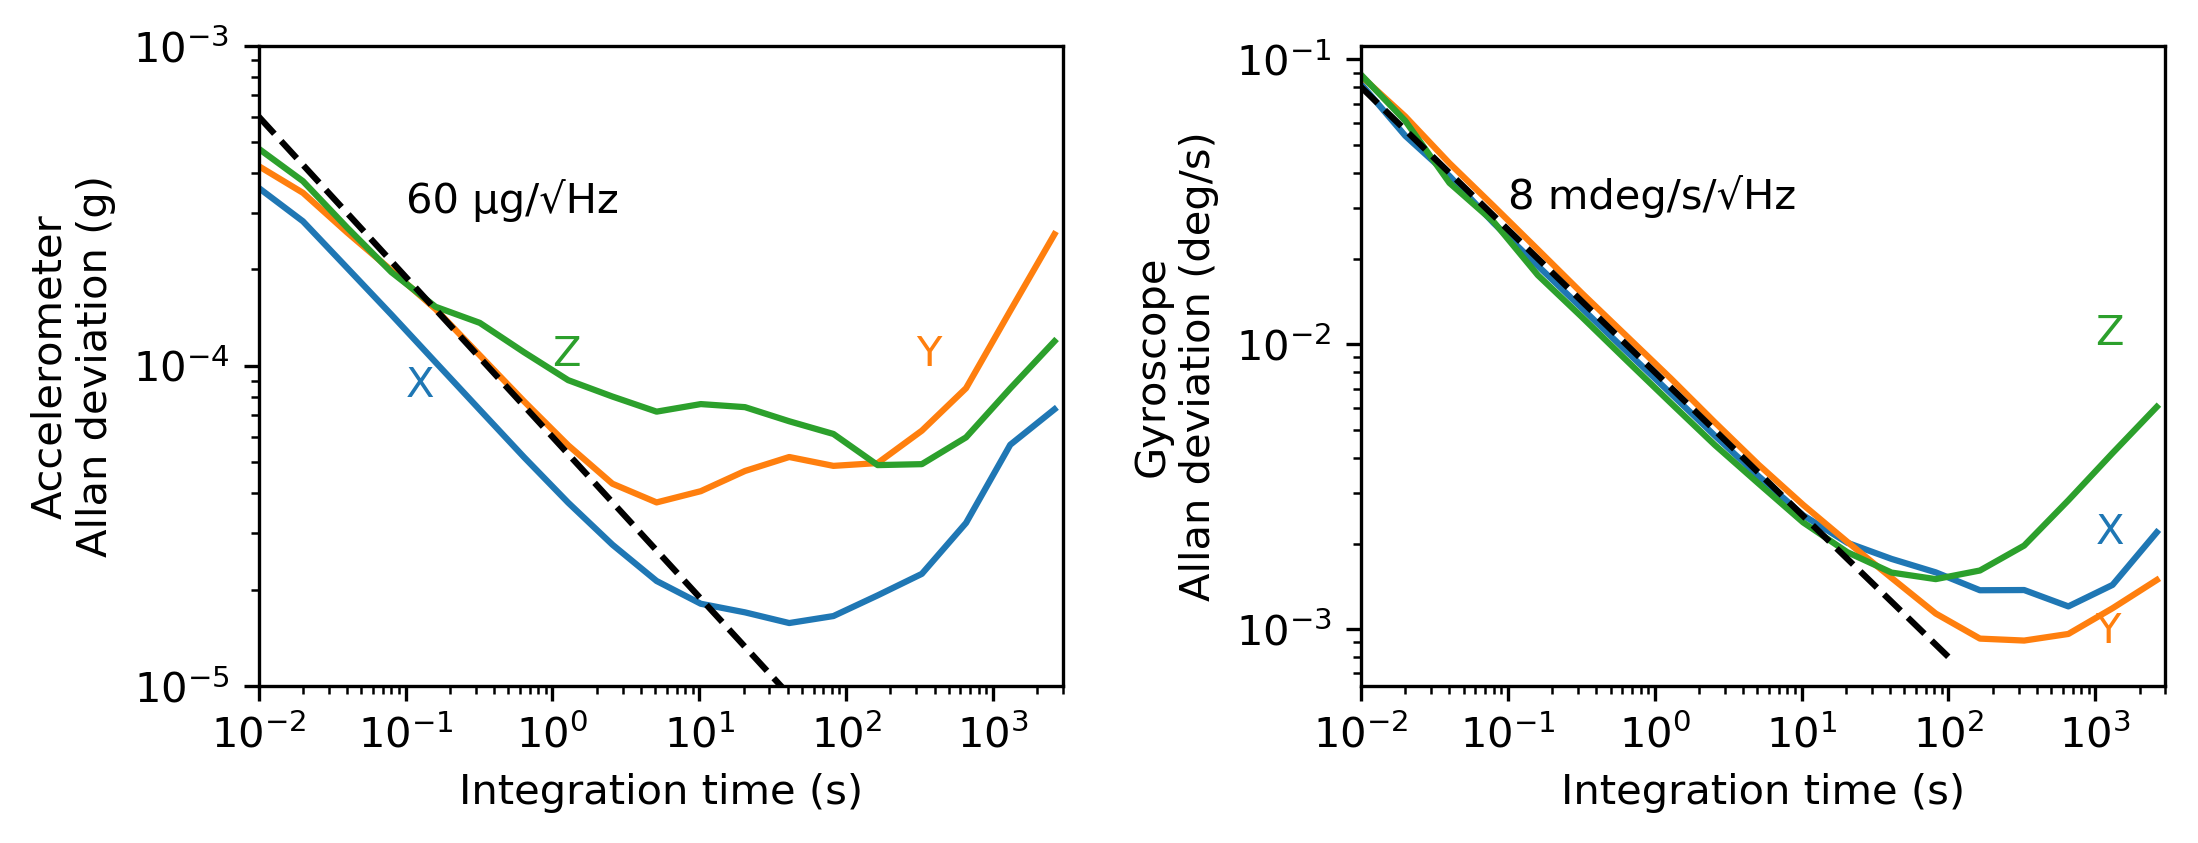
\includegraphics[width=\textwidth]{../images/allan-deviation2.png}
  \caption{\label{fig:allan-deviation} The Allan-deviation of the IMU sensors. The accelerometers all have a noise performance of \SI{60}{\micro g/\sqrt{Hz}} or better, and the gyroscopes have a noise performance of \SI{60}{mdeg/\sqrt{Hz}} or better.}
\end{figure}

\section{Kalman Filtering of an iPhone 8 in three dimensions}

We were not successful at producing a Kalman filter that accurately maintained the orientation of the iPhone 8 during field tests. The GNSS data was sufficient to cause the phone's location updates to converge somewhat close to the GNSS locations. Unfortunately, modeling error made the algorithm's estimate of the position unstable. Dozens of hours of effort were invested to isolate the problem, but without success.

The state of the most-recent Kalman filter implementation used in three dimensions is as follows 

\begin{equation}
\vec\mu = (r_x, r_y, r_z, v_x, v_y, v_z, \alpha, \beta, \gamma)^T
\end{equation}

where $\vec r$ corresponds to position and $\vec v$ corresponds to velocity in the global coordinate system.

\begin{equation}
\vec{u} = (a_X, a_Y, a_Z, \omega_Z, \omega_Y, \omega_Z)^T
\end{equation}

where $\omega_Z, \omega_Y, and \omega_Z$ represent incremental changes in the yaw, pitch, and roll in the aircraft frame respectively.

\def\dts{\frac{dt^2}{2}}
\def\sga{\sigma_a\sqrt{f_s}}
\def\sgg{\sigma_g\sqrt{f_s}}

\begin{equation}
Q = \left[ I_9 \left(\sga\dts, \sga\dts, \sga\dts, \sga dt, \sga dt, \sga dt, \sgg dt, \sgg dt \sgg dt \right)^T \right]^2
\end{equation}

Where the bandwidth $f_s$ is \SI{100}{Hz} and the value of $\sigma_a$ and $\sigma_g$ are determined from the Allan-deviation characterization to be \SI{60}{\micro g/\sqrt{Hz}} and \SI{8}{mdeg/\sqrt{Hz}} respectively.

The value of the diagonal elements of $S$ can be calculated at each timestep from the GNSS-sensor estimate of the horizontal and vertical accuracy provided by the iPhone API.

\begin{equation}
H = \begin{pmatrix}
1 & 0 & 0 & 0 & 0 & 0 & 0 & 0 & 0 \\
0 & 1 & 0 & 0 & 0 & 0 & 0 & 0 & 0 \\
0 & 0 & 1 & 0 & 0 & 0 & 0 & 0 & 0 \\
\end{pmatrix}
\end{equation}

\begin{equation}
P_0 = Q + S
\end{equation}

where once again, we have set the diagonal element in $P_0$ corresponding to the yaw to be $\pi^2$ to represent our lack of confidence in the value's initialization.

The equations of motion $f$ that govern the system are too complicated to be expressed concisely in a matrix form, and must be taken in steps. First, the orientation of the device is updated using the values from the previous state

\begin{equation}
R_{t} = R(\omega_Z, \omega_Y, \omega_Z) R(\alpha_{t-1}, \beta_{t-1}, \gamma_{t-1})
\end{equation}

\begin{align}
  \alpha_t &= \mathrm{atan2}(r_{21}, r_{22})\\
  \beta_t &= \mathrm{asin}(-r_{23}) \\ 
  \gamma_t &= \mathrm{atan}(r_{13}/r_{33})
\end{align}

Next, the acceleration in the global coordinate frame is calculated from a rotated version of the accelerometers 

\begin{equation}
  \vec{a} = 
\begin{pmatrix}
a_x \\ a_y \\ a_z 
\end{pmatrix}
=
[R(\alpha_{t-1}, \beta_{t-1}, \gamma_{t-1})]^T 
\begin{pmatrix}
a_X \\ a_Y \\ a_Z
\end{pmatrix}
+
\begin{pmatrix}
  0 \\ 0 \\ g
\end{pmatrix}  
\label{eq:accelerationconversion}
\end{equation}

where the addition of the final term corrects for the gravitational field of earth.

Finally, the position and velocity vectors are updated 

\begin{align}
\vec{r}_t &= \vec{r}_{t-1} + \vec{v}_{t-1} dt + \vec{a} dt^2/2 \\
\vec{v}_t &= \vec{v}_{t-1} + \vec{a} dt
\end{align}

The linearization of the above steps is somewhat involved and very prone to human error when done by hand. In the present work, the terms of the linearization of the calculation of $\alpha_t, \beta_t,$ and $\gamma_t$ are considered small to save us the work of linearizing the trigonometric functions of several terms. They are represented in the Jacobian matrix $F$ as $\epsilon$, but in the computational algorithm are treated as 0 for now.  To calculate the dependence of the position and velocity measurements as a function of the error in the orientation, we begin by referencing Eq. \ref{eq:rotationmatrix} and calculating the transpose.

\begin{equation}
  [R(\alpha, \beta, \gamma)]^T
  =
\begin{pmatrix}
  \ca\cg-\sa\sb\sg & \sa\cb & -\sa\sb\cg - \ca\sg \\ 
   -\sa\cg - \ca\sb\sg & \ca\cb & -\ca\sb\cg + \sa\sg \\
   \cb\sg&  -\sb& \cb\cg
  \end{pmatrix}
\end{equation}

Equation \ref{eq:accelerationconversion} becomes 

\begin{align}
  a_x &=   (\ca\cg-\sa\sb\sg) a_X + (\sa\cb) a_Y + (-\sa\sb\cg - \ca\sg) a_Z \\ 
  a_y &= (-\sa\cg - \ca\sb\sg) a_X + (\ca\cb)a_Y + (-\ca\sb\cg + \sa\sg) a_Z \\
  a_z &= (\cb\sg)a_X +  (-\sb)a_Y + (\cb\cg) a_Z + g
\end{align}

The first-order derivatives with respect to the Tait-Bryan angles are



%\begin{align}
  %\dd x\alpha &= (-\sa \cg -\ca\sb\sg, \ca \cb, -\ca\sb\cg+\sa\sg) \aa\\
  %\dd y\alpha &= (-\ca\cg+\sa\sb\sg, -\sa\cb, \sa\sb\cg+\ca\sg) \aa\\
  %\dd z\alpha &= 0
%\end{align}

\begin{equation}
  \frac{\partial}{\partial \alpha}
  \begin{pmatrix}
    a_x \\ a_y \\ a_z
  \end{pmatrix}
  = 
\begin{pmatrix}
  -\sa \cg -\ca\sb\sg & \ca \cb & -\ca\sb\cg+\sa\sg \\
 -\ca\cg+\sa\sb\sg & -\sa\cb &  \sa\sb\cg+\ca\sg \\
0 & 0 & 0
\end{pmatrix}
\begin{pmatrix}
a_X \\ a_Y \\ a_Z
\end{pmatrix}
\end{equation}

The row of zeros indicates that the global acceleration in the $z$ direction is not sensitive to $a_Z$ for errors in yaw 

\begin{equation}
  \frac{\partial}{\partial \beta}
  \begin{pmatrix}
    a_x \\ a_y \\ a_z
  \end{pmatrix}
  = 
\begin{pmatrix}
 -\sa\cb\sg & -\sa\sb & -\sa \cb \cg\\
 -\ca\cb\sg & -\ca\sb & -\ca\cb\cg \\
 -\sb\sg & -\cb & -\sb \cg\\
\end{pmatrix}
\begin{pmatrix}
a_X \\ a_Y \\ a_Z
\end{pmatrix}
\end{equation}

\begin{equation}
  \frac{\partial}{\partial \gamma}
  \begin{pmatrix}
    a_x \\ a_y \\ a_z
  \end{pmatrix}
  = 
\begin{pmatrix}
-\ca\sg -\sa\sb\cg & 0 & \sa\sb\sg - \ca\cg \\
\sa\sg - \ca\sb\cg & 0 & \ca\sb\sg + \sa\cg \\
\cb \cg & 0 & -\cb\sa  
\end{pmatrix}
\begin{pmatrix}
a_X \\ a_Y \\ a_Z
\end{pmatrix}
\end{equation}

The column of zeros signifies the error in global acceleration does not depend on the $a_Y$ accelerometer if the roll is varied.

Thus, the linearized vector $F$ is 
\newcommand\dd[2]{\dfrac{\partial a_{#1}}{\partial {#2}} }
\def\dts{\dfrac{dt^2}{2}}

\begin{equation}
F = \begin{pmatrix}
1 & 0 & 0 & dt & 0 & 0 & \dd x\alpha \dts & \dd x\beta \dts & \dd x\gamma \dts \\
0 & 1 & 0 & 0 & dt & 0 & \dd y\alpha \dts & \dd y\beta \dts & \dd y\gamma \dts \\
0 & 0 & 1 & 0 & 0 & dt & \dd z\alpha \dts & \dd z\beta \dts & \dd z\gamma \dts \\
0 & 0 & 0 & 1 & 0 & 0 & \dd x\alpha dt & \dd x \beta dt & \dd x \gamma dt \\
0 & 0 & 0 & 0 & 1 & 0 & \dd y\alpha dt & \dd y \beta dt & \dd y \gamma dt \\
0 & 0 & 0 & 0 & 0 & 1 & \dd z\alpha dt & \dd z \beta dt & \dd z \gamma dt \\
0 & 0 & 0 & 0 & 0 & 0 & 1 & \epsilon_1 & \epsilon_2  \\
0 & 0 & 0 & 0 & 0 & 0 & \epsilon_4 & 1 & \epsilon_4  \\
0 & 0 & 0 & 0 & 0 & 0 & \epsilon_5 & \epsilon_6 & 1  \\
\end{pmatrix}
\end{equation}

In software implementations, because no analytic solution to the six values of $\epsilon$ was derived, they were treated as zero. The Kalman filter was, however, programmed with a second update step (in addition to the GNSS update). In this update step, which only occurred when the magnitude of the total acceleration was close to $g$ (i.e., $a_X^2 + a_Y^2 + a_Z^2 \approx g^2$), the Kalman filter assumed that the device was not accelerating, and that the direction of the total acceleration was equivalent to the direction of the gravity vector. This allowed for an update to the pitch and the roll of the device. For this correction, 

\begin{equation}
  h(\vec\mu) = R(\alpha, \beta, \gamma) (0, 0, -g)
\end{equation}

which, when linearized is

\begin{equation}
H = g\begin{pmatrix}
0 & 0 & 0& 0& 0& 0& 0& \sb\sg & -\cb\cg \\
0 & 0 & 0& 0& 0& 0& 0& \cb & 0 \\
0 & 0 & 0& 0& 0& 0& 0& -\sb\cg & -\cb\sg \\
\end{pmatrix}
\vec \mu
\end{equation}

The value of $z$ was $(a_X, a_Y, a_Z)^T$, and the value of $S$ was estimated by the magnitude of $(a_X^2 + a_Y^2 + a_Z^2)/g^2 - 1$

\begin{figure}
  \centering
  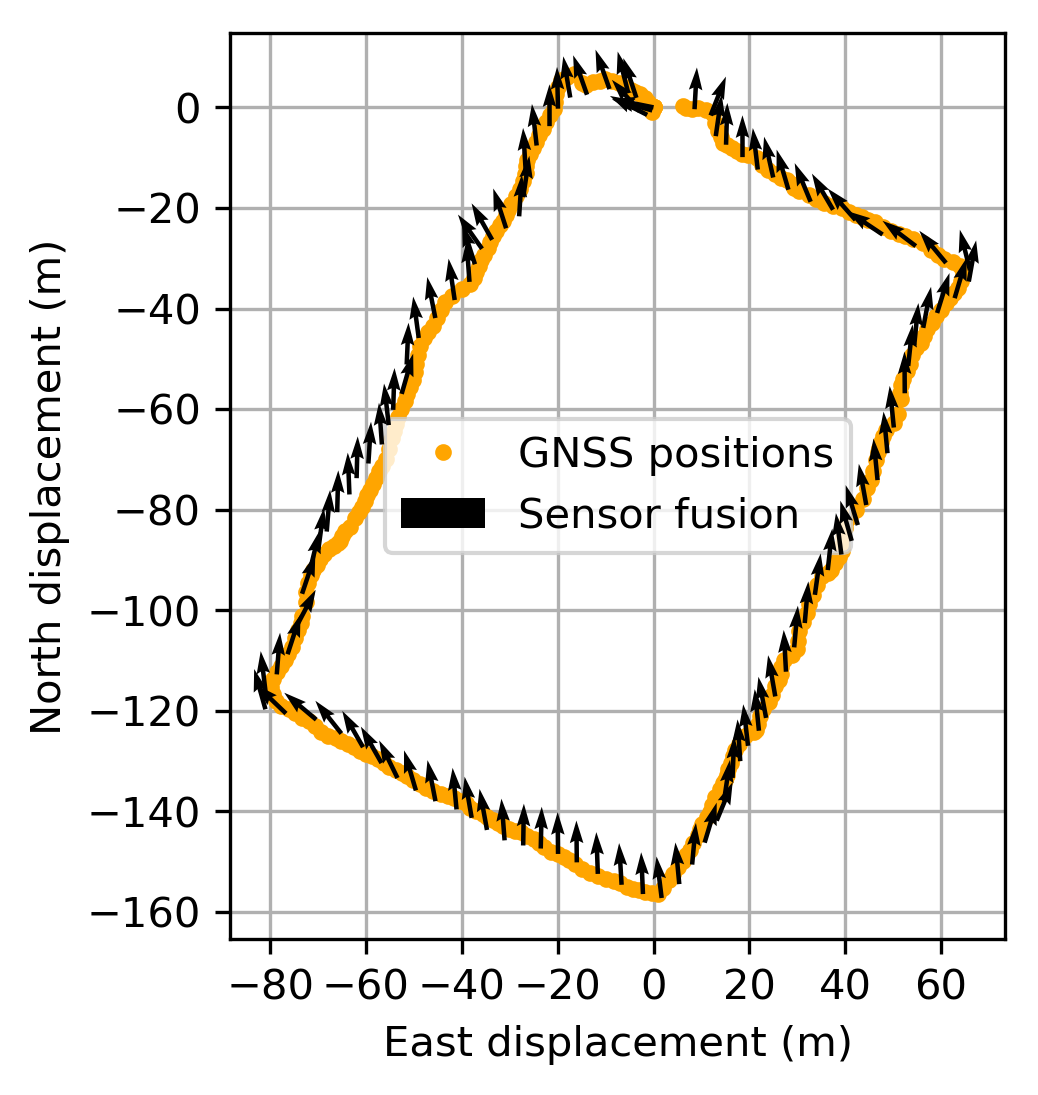
\includegraphics[height=3in]{../images/walk-around-block.png}
  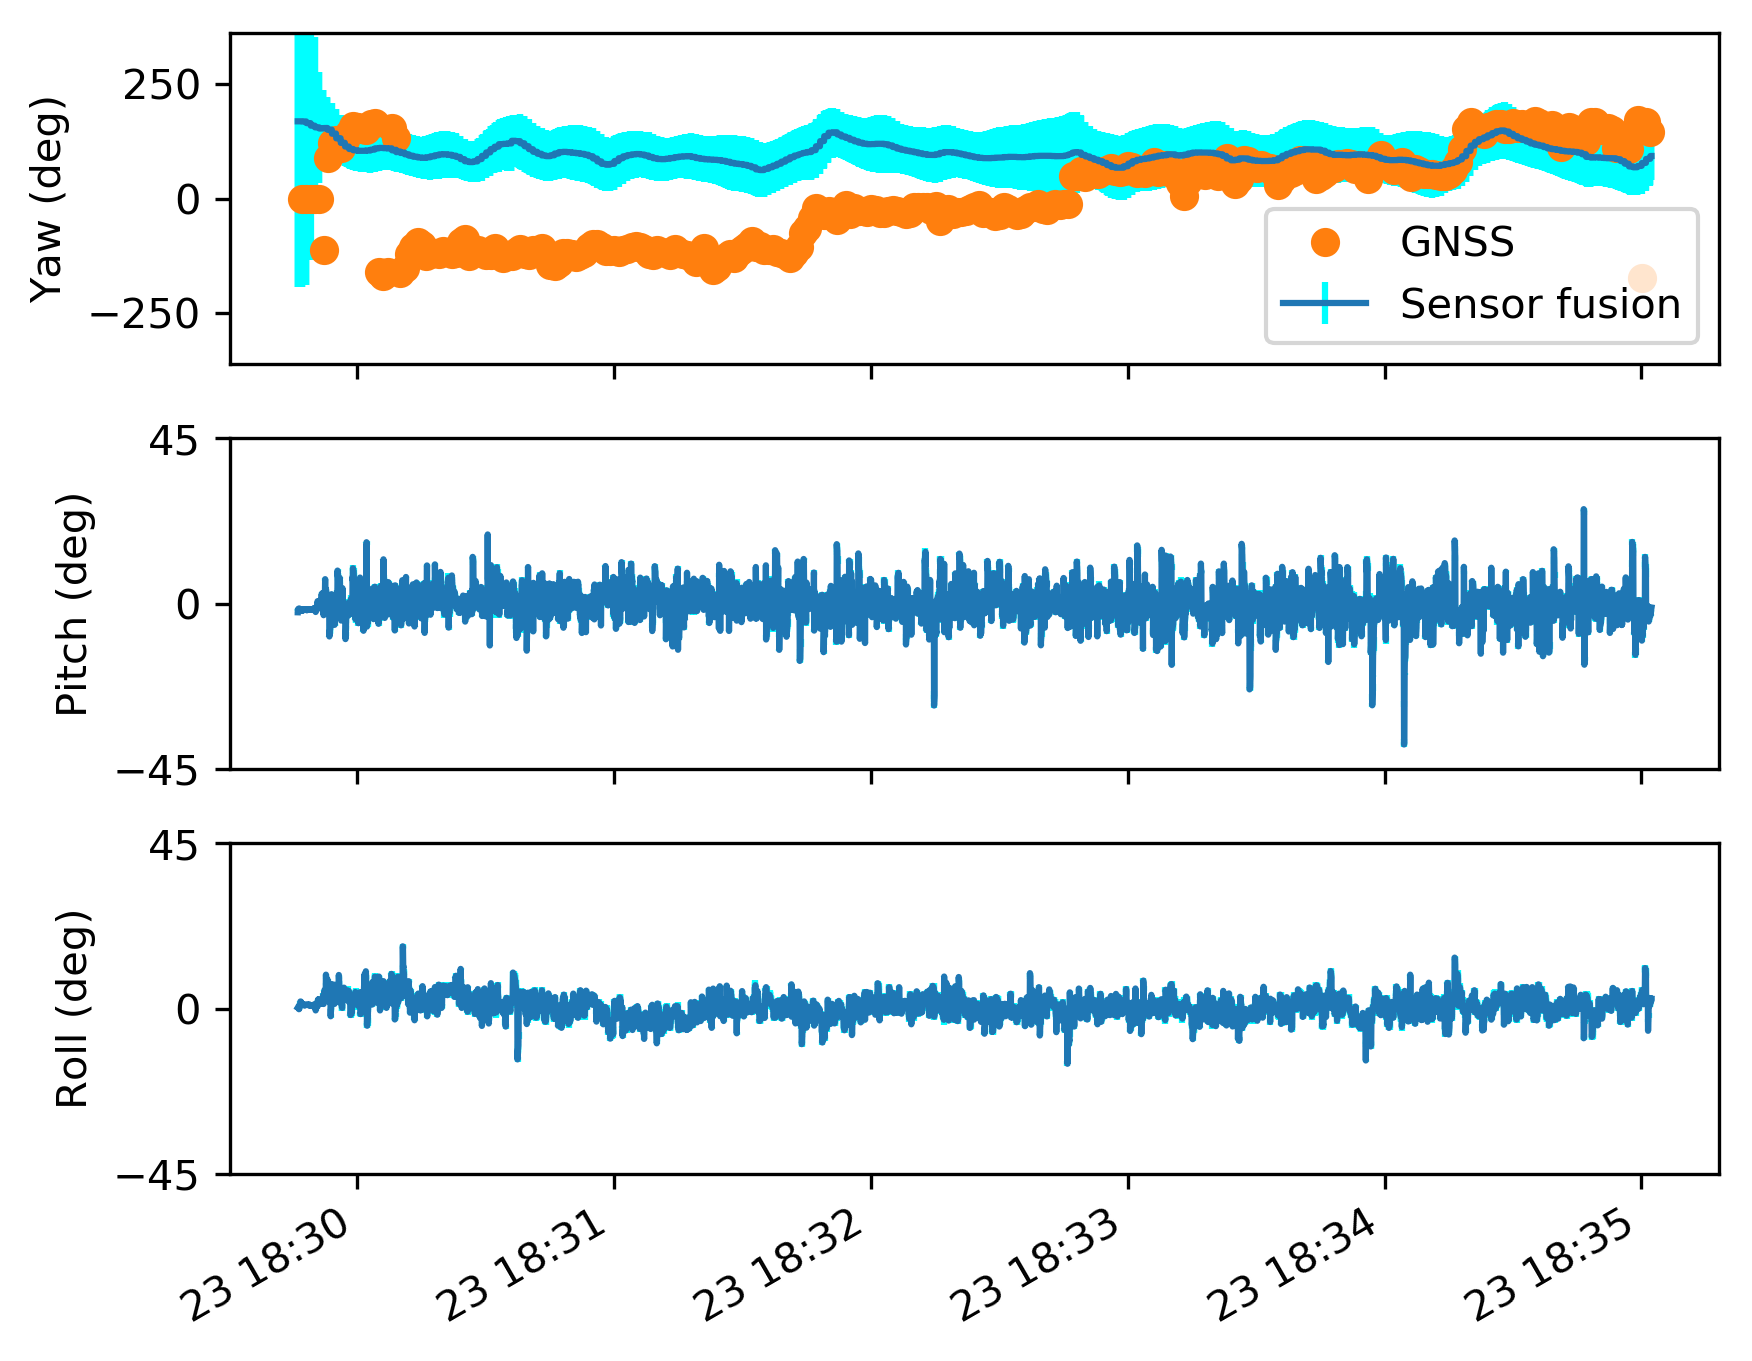
\includegraphics[height=3in]{../images/time-trace-of-bike-path.png}
  \caption{\label{fig:bikewalk} Left: a birds-eye view of the trajectory taken during the field test. The path started near the top of the curve, and followed the rectangular path counter-clockwise. The orange dots represent position estimates of the GNSS sensor, and the black arrows represent locations and orientations of the phone as estimated by the Kalman filter. Right: Three time traces of the Kalman filter's estimate of yaw, pitch, and roll. The orange dots in the top chart represent the heading (yaw) estimate based on the difference between subsequent GNSS updates. The error bars are plotted in cyan.}
\end{figure}

To test the filter, an iPhone was placed on the seat of a bicycle so that it's $Y$ direction faced towards the front of the bicycle. The $X$ direction was facing to the right of the bicycle, and the $Z$ direction was pointing straight up into the sky. The bicycle was walked at a constant speed clockwise around one city block. The results of this test are shown in Fig. \ref{fig:bikewalk}.

The Kalman filter proved to be very unstable. When the values of the Q matrix were small (corresponding to low-noise in the IMU sensors), the algorithm ignored updates from the GNSS sensor. In early debugging attempts, the position estimates quickly diverged from the local neighborhood and the phone's estimated position left the bay area and departed into outer space. This was likely due to some errors in how the Kalman filter corrects for orientation.

In order to get the sensor-fusion position estimates to be somewhat close to the GNSS positions, the Q matrix had to be updated to reflect large noise in the accelerometers. Thus, the algorithm trusted the GNSS updates more than the IMU sensors, and the error converged to the sidewalk upon which the bicycle was moving.

Even then, the estimates for the heading of the device did not seem to track the ground truth. The phone was always positioned in the direction of travel, so the arrows in Fig. \ref{fig:bikewalk} should have been pointing parallel to the direction of travel. Instead, the arrows in Fig. \ref{fig:bikewalk} seem to point mostly north, and do not seem to be obviously correlated with the path direction or any other test quantity.

The pitch and the roll, on the other hand, converged nicely. However, this is because these two quantities were determined by a feedback correction mechanisms (using an calculation that predicts these values through $z - h(\vec \mu)$ instead of $f(\vec\mu, \vec u)$). There are no visible error bars in Fig. \ref{fig:bikewalk}, and the ``noise'' in pitch represent bumps in the aging sidewalks where the test was performed, and the drift in the roll represent the fact that the bicycle leaned a little to the right and a little to the left as it was pushed around the block.

As mentioned previously, the instability of this filter and its overall failure to correctly calculate the heading (yaw) correctly are likely due to a failure to derive and linearize the equations of motion correctly. The linearized $F$ matrix contains no fewer than 29 non-zero terms. In principle, all 29 of these terms need to be calculated correctly in order for the filter to perform as required. Furthermore, to save on mathematical complexity, the calculation of the pitch and roll was performed by comparing the accelerometer vector to the gravity vector in a feedback step, rather than propagating the uncertainties a predict step. As has been seen in previous sections, most of the code used in the Kalman filter software implementation functions correctly, but likely a few signs were flipped or a derivative was misapplied in the calculation of $F$ which caused the system to become unstable. Further debugging is likely to uncover the source of the problem, and then the sensor would perform optimally, yielding errors of less than a meter without having to artificially increase the values of $Q$ to minimize IMU drift.

\section{Conclusion}

We have demonstrated EKFs suitable for tracking the motion and orientation of objects in one, two and three dimensions. The EKFs make use of IMU sensor data and are corrected periodically by measurements from a GNSS sensor. These EKFs are also tested using the IMU and GNSS chips in an iPhone 8 using trajectories that a typical pedestrian might experience.

In principle, the construction of an EKF is straightforward, but prone to human errors. The equations that govern the laws of motion involve significant amounts of trigonometry, and deriving the Jacobian of the state evolution function by hand includes dozens of terms. If any of these terms is incorrect or takes the wrong sign, the EKF is no longer stable and causes the estimation of the state to quickly diverge from the true state. 

Furthermore, the approach used to track the device orientation makes use of a yaw-pitch-roll coordinate frame which becomes degenerate (due to gimbal lock) when the device is either vertically up or down. This causes large numerical instabilities when the device is in these orientations (e.g., the user is taking a picture of some object at eye-level, or the device is in the user's pocket). An alternative solution implements quaternions, though this comes at the added challenge of linearizing the rotation operations between the IMU's reference frame and the global reference frame.

\subsection{Further Work}

The performance of these Kalman filters could further be enhanced by accounting for other forces (such as centripetal acceleration and the Coriolis force) in the state-evolution equations in the Kalman filter.

Each of the gyroscopes and accelerometers has some offset that varies with time. A high-performance Kalman filter would include six additional terms in its state model to estimate the gyroscope and accelerometer biases. While the bias of any given sensor can be modeled somewhat using a knowledge of the temperature and magnetic field at the sensor, some of the offset drift still is difficult to develop a physical model for, but the expectation value of its rate of its drift over time can be characterized experimentally and used to define the process noise for its associated $Q$-matrix values.

The iPhone API does not expose the pseudorange measurements used to calculate the GNSS latitude, longitude, and altitude. It merely provides a latitude, longitude, altitude, horizontal accuracy, and vertical accuracy. In principle, an EKF would have superior performance (even in urban environments where only one or two satellites may be available) by using $h(\vec{\mu})$ to calculate the expected pseudoranges to each satellite, and comparing $h(\vec{\mu})$ to the measured pseudoranges $\vec{z}$. This algorithm is similar to the gradient-descent algorithm already used to estimate the GNSS position, except that in the absence of IMU data, four pseudoranges are required to estimate $x, y, z$, and $t$. The data in an EKF can ease this 4-satellite constraint. In urban environments, this would help bound the vertical error, which already is somewhat unstable due to the numerical difficulty of canceling out the earth's gravitational bias on the z-accelerometer.

\bibliographystyle{ieeetr}  
%\bibliographystyle{unsrt}
\bibliography{bib} 

\end{document}   